\chapter{Risultati Numerici Completi}
\label{app:risultati_completi}

La presente appendice raccoglie i risultati numerici completi associati alle analisi sperimentali sviluppate nel Capitolo~\ref{ch:risultati}.
Al fine di preservare la leggibilità della discussione principale, nel Capitolo~\ref{ch:risultati} sono riportati i risultati necessari all'interpretazione e al confronto tra i paradigmi sperimentali, mentre nel seguito sono raccolti i relativi dettagli numerici completi.

L'organizzazione dell'appendice segue la medesima articolazione logica adottata nell'analisi sperimentale: baseline \texttt{INJECTION}, modelli sorgente, modelli ibridi e verifiche statistiche.


% ==============================================================================
% BASELINE
% ==============================================================================

\section{Risultati Completi della Baseline INJECTION}
\label{app:baseline_injection}

La presente sezione raccoglie il dettaglio numerico delle valutazioni della baseline \texttt{INJECTION} discusse nella Sezione~\ref{sec:baseline_prestazioni}. 
Sono riportate separatamente le cardinalità complete delle matrici di confusione e le metriche complementari ottenute sui benchmark di cross-evaluation.

\subsection{Matrici di Confusione}

La Tabella~\ref{tab:baseline_confusion_seed42} riporta le cardinalità complete delle matrici di confusione ottenute dalla baseline \texttt{INJECTION} con i classificatori DT, HGB e RF sui $16$ test set considerati per il seed $s=42$.

\begin{table}[H]
    \centering
    \footnotesize
    \caption{Cardinalità complete delle matrici di confusione della baseline \texttt{INJECTION} con DT, HGB e RF sui $16$ test set per il seed $s=42$.}
    \label{tab:baseline_confusion_seed42}
    \resizebox{\textwidth}{!}{
    \begin{tabular}{lcccc|cccc|cccc}
        \toprule
        & \multicolumn{4}{c|}{\textbf{DT}} & \multicolumn{4}{c|}{\textbf{HGB}} & \multicolumn{4}{c}{\textbf{RF}} \\
        \textbf{Test Set} & \textbf{TP} & \textbf{TN} & \textbf{FP} & \textbf{FN} & \textbf{TP} & \textbf{TN} & \textbf{FP} & \textbf{FN} & \textbf{TP} & \textbf{TN} & \textbf{FP} & \textbf{FN} \\
        \midrule
        \texttt{nb15} (aggregato) & 1539 & 18305 & 295 & 321 & 1482 & 18540 & 60 & 378 & 1530 & 18422 & 178 & 330 \\
        \texttt{nb15} (DoS) & 1693 & 18305 & 295 & 167 & 1648 & 18540 & 60 & 212 & 1705 & 18422 & 178 & 155 \\
        \texttt{nb15} (Exploits) & 1567 & 18305 & 295 & 293 & 1522 & 18540 & 60 & 338 & 1598 & 18422 & 178 & 262 \\
        \texttt{nb15} (Fuzzers) & 525 & 18305 & 295 & 1335 & 338 & 18540 & 60 & 1522 & 450 & 18422 & 178 & 1410 \\
        \texttt{nb15} (Generic) & 1843 & 18305 & 295 & 17 & 1843 & 18540 & 60 & 17 & 1843 & 18422 & 178 & 17 \\
        \texttt{nb15} (Reconnaissance) & 1619 & 18305 & 295 & 241 & 1642 & 18540 & 60 & 218 & 1596 & 18422 & 178 & 264 \\
        \texttt{injection} (aggregato) & 1535 & 18305 & 295 & 325 & 1506 & 18540 & 60 & 354 & 1531 & 18422 & 178 & 329 \\
        \texttt{nb15\_stin} (aggregato) & 1790 & 18305 & 295 & 70 & 1405 & 18540 & 60 & 455 & 1851 & 18422 & 178 & 9 \\
        \texttt{nb15\_sat20} (aggregato) & 1841 & 18305 & 295 & 19 & 1589 & 18540 & 60 & 271 & 1859 & 18422 & 178 & 1 \\ 
        \texttt{nb15\_sat20} (Syn\_DDoS) & 1825 & 18305 & 295 & 35 & 1512 & 18540 & 60 & 348 & 1860 & 18422 & 178 & 0 \\
        \texttt{nb15\_sat20} (UDP\_DDoS) & 1859 & 18305 & 295 & 1 & 1672 & 18540 & 60 & 188 & 1859 & 18422 & 178 & 1 \\
        \texttt{nb15\_ter20} (aggregato) & 1752 & 18305 & 295 & 108 & 1295 & 18540 & 60 & 565 & 1842 & 18422 & 178 & 18 \\
        \texttt{nb15\_ter20} (Botnet) & 1636 & 18305 & 295 & 224 & 1498 & 18540 & 60 & 362 & 1857 & 18422 & 178 & 3 \\
        \texttt{nb15\_ter20} (DDoS) & 1860 & 18305 & 295 & 0 & 1539 & 18540 & 60 & 321 & 1860 & 18422 & 178 & 0 \\
        \texttt{nb15\_ter20} (Syn\_DDoS) & 1794 & 18305 & 295 & 66 & 0 & 18540 & 60 & 1860 & 1731 & 18422 & 178 & 129 \\
        \texttt{nb15\_ter20} (UDP\_DDoS) & 1664 & 18305 & 295 & 196 & 1286 & 18540 & 60 & 574 & 1860 & 18422 & 178 & 0 \\
        \bottomrule
    \end{tabular}
    }
\end{table}

\subsection{Metriche Complementari}

La Tabella~\ref{tab:baseline_f1_prauc_seed42} completa la caratterizzazione della baseline riportando i valori di \textit{F1-Score} e PR-AUC ottenuti dai tre classificatori sui medesimi $16$ test set per il seed $s=42$.

\begin{table}[H]
    \centering
    \footnotesize
    \caption{F1-Score e PR-AUC completi della baseline \texttt{INJECTION} con DT, HGB e RF sui $16$ test set per il seed $s=42$.}
    \label{tab:baseline_f1_prauc_seed42}
    \resizebox{\textwidth}{!}{
    \begin{tabular}{lcc|cc|cc}
        \toprule
        & \multicolumn{2}{c|}{\textbf{DT}} & \multicolumn{2}{c|}{\textbf{HGB}} & \multicolumn{2}{c}{\textbf{RF}} \\
        \textbf{Test Set} & \textbf{F1-Score} & \textbf{PR-AUC} & \textbf{F1-Score} & \textbf{PR-AUC} & \textbf{F1-Score} & \textbf{PR-AUC} \\
        \midrule
        \texttt{nb15} (aggregato) & 0.8332 & 0.7120 & 0.8713 & 0.9263 & 0.8576 & 0.9095 \\
        \texttt{nb15} (DoS) & 0.8799 & 0.7548 & 0.9238 & 0.9648 & 0.9110 & 0.9602 \\
        \texttt{nb15} (Exploits) & 0.8420 & 0.7102 & 0.8844 & 0.9469 & 0.8790 & 0.9342 \\
        \texttt{nb15} (Fuzzers) & 0.3918 & 0.2890 & 0.2994 & 0.5824 & 0.3617 & 0.5099 \\
        \texttt{nb15} (Generic) & 0.9220 & 0.8571 & 0.9795 & 0.9968 & 0.9498 & 0.9932 \\
        \texttt{nb15} (Reconnaissance) & 0.8580 & 0.7053 & 0.9220 & 0.9659 & 0.8784 & 0.9461 \\
        \texttt{injection} (aggregato) & 0.8320 & 0.7104 & 0.8792 & 0.9342 & 0.8579 & 0.9154 \\
        \texttt{nb15\_stin} (aggregato) & 0.9075 & 0.8316 & 0.8451 & 0.9191 & 0.9519 & 0.9802 \\
        \texttt{nb15\_sat20} (aggregato) & 0.9214 & 0.8560 & 0.9057 & 0.9579 & 0.9541 & 0.9873 \\
        \texttt{nb15\_sat20} (Syn\_DDoS) & 0.9171 & 0.8484 & 0.8811 & 0.9682 & 0.9543 & 0.9902 \\
        \texttt{nb15\_sat20} (UDP\_DDoS) & 0.9263 & 0.8646 & 0.9310 & 0.9604 & 0.9541 & 0.9898 \\
        \texttt{nb15\_ter20} (aggregato) & 0.8969 & 0.8134 & 0.8056 & 0.8922 & 0.9495 & 0.9746 \\
        \texttt{nb15\_ter20} (Botnet) & 0.8631 & 0.7581 & 0.8765 & 0.9464 & 0.9535 & 0.9675 \\
        \texttt{nb15\_ter20} (DDoS) & 0.9265 & 0.8651 & 0.8899 & 0.9379 & 0.9543 & 0.9834 \\
        \texttt{nb15\_ter20} (Syn\_DDoS) & 0.9086 & 0.8339 & 0.0000 & 0.5501 & 0.9185 & 0.9660 \\
        \texttt{nb15\_ter20} (UDP\_DDoS) & 0.8714 & 0.7714 & 0.8022 & 0.9499 & 0.9543 & 0.9859 \\
        \bottomrule
    \end{tabular}
    }
\end{table}



% ==============================================================================
% MODELLI SORGENTE
% ==============================================================================

\section{Risultati Completi dei Modelli Sorgente}
\label{app:modelli_sorgente}

La presente sezione raccoglie il dettaglio numerico delle analisi relative ai modelli addestrati esclusivamente sul dominio sorgente, discusse nella Sezione~\ref{sec:risultati_modelli_sorgente}. 
I risultati sono organizzati distinguendo le prestazioni sul dominio sorgente, la risposta cross-domain, la specificità multi-seed e il confronto con la baseline \texttt{INJECTION}.

% ==============================================================================
% RISULTATI COMPLETI DEI MODELLI SORGENTE
% ==============================================================================

\subsection{Prestazioni sul Dominio Sorgente e su INJECTION}

La Tabella~\ref{tab:sorgente_mean_tpr_source_tests} sintetizza la TPR media calcolata sui $10$ seed per i modelli sorgente, considerando le valutazioni effettuate sui benchmark appartenenti al dominio sorgente e sul test set \texttt{INJECTION}.

\begin{table}[H]
    \centering
    \footnotesize
    \caption{TPR media sui $10$ seed dei modelli sorgente valutati sui benchmark sorgente e sul test set \texttt{INJECTION}.}
    \label{tab:sorgente_mean_tpr_source_tests}
    \resizebox{\textwidth}{!}{
    \begin{tabular}{lccccccc}
        \toprule
        \textbf{Modello} & \textbf{Aggr. NB15} & \textbf{DoS} & \textbf{Exploits} & \textbf{Fuzzers} & \textbf{Generic} & \textbf{Recon.} & \textbf{INJECTION} \\
        \midrule
        \multicolumn{8}{c}{\textbf{DT}} \\
        \hline
        Aggregato      & 0.8215 & 0.9073 & 0.8432 & 0.2851 & 0.9916 & 0.8737 & 0.8274 \\
        DoS            & 0.5908 & 0.9306 & 0.7211 & 0.1725 & 0.6300 & 0.2015 & 0.5847 \\
        Exploits       & 0.3942 & 0.9261 & 0.8927 & 0.1903 & 0.0220 & 0.2504 & 0.4167 \\
        Fuzzers        & 0.3197 & 0.7847 & 0.4175 & 0.4794 & 0.0805 & 0.1906 & 0.3201 \\
        Generic        & 0.6042 & 0.7359 & 0.4273 & 0.1213 & 0.9867 & 0.1421 & 0.5972 \\
        Reconnaissance & 0.6592 & 0.7911 & 0.4459 & 0.1450 & 0.9444 & 0.9386 & 0.6627 \\
        \hline
        \multicolumn{8}{c}{\textbf{HGB}} \\
        \hline
        Aggregato      & 0.8018 & 0.8941 & 0.8173 & 0.1775 & 0.9900 & 0.8797 & 0.8039 \\
        DoS            & 0.7029 & 0.9131 & 0.7357 & 0.1391 & 0.9648 & 0.1933 & 0.7048 \\
        Exploits       & 0.4278 & 0.9099 & 0.8714 & 0.1629 & 0.1310 & 0.2248 & 0.4442 \\
        Fuzzers        & 0.2524 & 0.7605 & 0.3610 & 0.3517 & 0.0089 & 0.1470 & 0.2520 \\
        Generic        & 0.5454 & 0.5847 & 0.3317 & 0.0913 & 0.9879 & 0.1095 & 0.5426 \\
        Reconnaissance & 0.6724 & 0.7794 & 0.4054 & 0.1375 & 0.9785 & 0.9465 & 0.6671 \\
        \hline
        \multicolumn{8}{c}{\textbf{RF}} \\
        \hline
        Aggregato      & 0.8236 & 0.9261 & 0.8619 & 0.2337 & 0.9915 & 0.8629 & 0.8272 \\
        DoS            & 0.7164 & 0.9320 & 0.7305 & 0.1487 & 0.9874 & 0.2039 & 0.7202 \\
        Exploits       & 0.3991 & 0.9282 & 0.9047 & 0.1750 & 0.0224 & 0.2386 & 0.4147 \\
        Fuzzers        & 0.3007 & 0.7704 & 0.3906 & 0.4739 & 0.0459 & 0.1669 & 0.2950 \\
        Generic        & 0.5792 & 0.7169 & 0.3621 & 0.1159 & 0.9870 & 0.1373 & 0.5694 \\
        Reconnaissance & 0.6602 & 0.7832 & 0.4235 & 0.1410 & 0.9580 & 0.9406 & 0.6621 \\
        \bottomrule
    \end{tabular}
    }
\end{table}


\subsection{Prestazioni Cross-Domain}

La Tabella~\ref{tab:sorgente_mean_tpr_target_tests} riporta la TPR media sui $10$ seed ottenuta dai modelli sorgente nella valutazione cross-domain sui benchmark target, distinguendo le configurazioni aggregate da quelle biclasse.

\begin{table}[H]
    \centering
    \footnotesize
    \caption{TPR media sui $10$ seed dei modelli sorgente valutati sui benchmark target aggregati e biclasse.}
    \label{tab:sorgente_mean_tpr_target_tests}
    \resizebox{\textwidth}{!}{
    \begin{tabular}{lccccccccc}
        \toprule
        \textbf{Modello} & \textbf{STIN} & \textbf{SAT20} & \textbf{TER20} & \textbf{SAT Syn} & \textbf{SAT UDP} & \textbf{Botnet} & \textbf{DDoS} & \textbf{TER Syn} & \textbf{TER UDP} \\
        \midrule
        \multicolumn{10}{c}{\textbf{DT}} \\
        \hline
        Aggregato      & 0.3807 & 0.1947 & 0.5294 & 0.0725 & 0.2917 & 0.6726 & 0.6669 & 0.0484 & 0.0538 \\
        DoS            & 0.4824 & 0.8149 & 0.2537 & 0.9528 & 0.6946 & 0.1320 & 0.0848 & 0.6024 & 0.8877 \\
        Exploits       & 0.2033 & 0.2978 & 0.1455 & 0.0715 & 0.4973 & 0.3573 & 0.0673 & 0.0284 & 0.0406 \\
        Fuzzers        & 0.4181 & 0.3712 & 0.4698 & 0.0178 & 0.6797 & 0.8898 & 0.4467 & 0.0092 & 0.0191 \\
        Generic        & 0.1267 & 0.3068 & 0.0141 & 0.0485 & 0.5289 & 0.0057 & 0.0118 & 0.0039 & 0.0459 \\
        Reconnaissance & 0.0501 & 0.0044 & 0.0812 & 0.0000 & 0.0063 & 0.0988 & 0.0079 & 0.3774 & 0.0000 \\
        \hline
        \multicolumn{10}{c}{\textbf{HGB}} \\
        \hline
        Aggregato      & 0.0662 & 0.1055 & 0.0438 & 0.0000 & 0.2020 & 0.0906 & 0.0378 & 0.0000 & 0.0000 \\
        DoS            & 0.1380 & 0.1540 & 0.1436 & 0.0000 & 0.2921 & 0.2309 & 0.1578 & 0.0000 & 0.0000 \\
        Exploits       & 0.0428 & 0.0287 & 0.0547 & 0.0000 & 0.0527 & 0.1013 & 0.0536 & 0.0000 & 0.0000 \\
        Fuzzers        & 0.2781 & 0.2157 & 0.3301 & 0.0000 & 0.4071 & 0.6226 & 0.3009 & 0.0000 & 0.0000 \\
        Generic        & 0.1137 & 0.2625 & 0.0204 & 0.0000 & 0.5016 & 0.0703 & 0.0006 & 0.0000 & 0.0000 \\
        Reconnaissance & 0.0005 & 0.0002 & 0.0000 & 0.0000 & 0.0001 & 0.0001 & 0.0001 & 0.0000 & 0.0000 \\
        \hline
        \multicolumn{10}{c}{\textbf{RF}} \\
        \hline
        Aggregato      & 0.3601 & 0.2613 & 0.4564 & 0.0000 & 0.4929 & 0.5570 & 0.6036 & 0.0000 & 0.0000 \\
        DoS            & 0.3558 & 0.6878 & 0.1296 & 0.5753 & 0.8007 & 0.1061 & 0.0594 & 0.1293 & 0.5109 \\
        Exploits       & 0.1594 & 0.3199 & 0.0522 & 0.0000 & 0.6077 & 0.1314 & 0.0355 & 0.0000 & 0.0000 \\
        Fuzzers        & 0.5040 & 0.4818 & 0.5338 & 0.0000 & 0.9023 & 0.9191 & 0.5841 & 0.0000 & 0.0000 \\
        Generic        & 0.1089 & 0.2572 & 0.0139 & 0.0000 & 0.4856 & 0.0448 & 0.0054 & 0.0000 & 0.0000 \\
        Reconnaissance & 0.0050 & 0.0156 & 0.0000 & 0.0000 & 0.0200 & 0.0029 & 0.0001 & 0.0000 & 0.0000 \\
        \bottomrule
    \end{tabular}
    }
\end{table}


\subsection{Specificità Multi-Seed}

La Tabella~\ref{tab:sorgente_tnr_multiseed} riporta la media e la varianza della TNR calcolate sui $10$ seed per ciascuna configurazione sorgente e per i tre classificatori considerati.

\begin{table}[H]
    \centering
    \footnotesize
    \caption{Media e varianza della TNR sui $10$ seed per i modelli sorgente. Il valore è indipendente dal test set malevolo poiché la componente nominale rimane invariata all'interno del protocollo sperimentale.}
    \label{tab:sorgente_tnr_multiseed}
    \begin{tabular}{lcc|cc|cc}
        \toprule
        & \multicolumn{2}{c|}{\textbf{DT}} & \multicolumn{2}{c|}{\textbf{HGB}} & \multicolumn{2}{c}{\textbf{RF}} \\
        \textbf{Modello} & $\boldsymbol{\overline{TNR}}$ & $\boldsymbol{\mathrm{Var}(TNR)}$ & $\boldsymbol{\overline{TNR}}$ & $\boldsymbol{\mathrm{Var}(TNR)}$ & $\boldsymbol{\overline{TNR}}$ & $\boldsymbol{\mathrm{Var}(TNR)}$ \\
        \midrule
        Aggregato & 0.98317 & $1.51\times10^{-7}$ & 0.99659 & $2.32\times10^{-8}$ & 0.99150 & $6.00\times10^{-8}$ \\
        DoS & 0.99362 & $5.51\times10^{-8}$ & 0.99776 & $5.38\times10^{-8}$ & 0.99672 & $8.44\times10^{-9}$ \\
        Exploits & 0.99049 & $4.99\times10^{-8}$ & 0.99588 & $7.07\times10^{-8}$ & 0.99413 & $2.46\times10^{-8}$ \\
        Fuzzers & 0.96248 & $1.77\times10^{-7}$ & 0.98900 & $2.38\times10^{-7}$ & 0.96847 & $8.01\times10^{-8}$ \\
        Generic & 0.99950 & $2.22\times10^{-9}$ & 0.99960 & $8.89\times10^{-9}$ & 0.99964 & $2.67\times10^{-9}$ \\
        Reconnaissance & 0.99521 & $1.21\times10^{-8}$ & 0.99555 & $7.17\times10^{-8}$ & 0.99608 & $1.51\times10^{-8}$ \\
        \bottomrule
    \end{tabular}
\end{table}


\subsection{Confronto Completo con la Baseline INJECTION}

La Tabella~\ref{tab:source_vs_base_target_variance} confronta la media e la varianza della TPR ottenute sui benchmark target aggregati dal modello sorgente aggregato e dalla baseline \texttt{INJECTION}, separatamente per DT, HGB e RF.

\begin{table}[H]
    \centering
    \footnotesize
    \caption{Media e varianza della TPR sui benchmark target aggregati per il modello sorgente aggregato e la baseline.}
    \label{tab:source_vs_base_target_variance}
    \begin{tabularx}{\textwidth}{l >{\centering\arraybackslash}X >{\centering\arraybackslash}X >{\centering\arraybackslash}X >{\centering\arraybackslash}X}
        \toprule
        & \multicolumn{2}{c}{\textbf{Modello sorgente}} & \multicolumn{2}{c}{\textbf{Baseline INJECTION}} \\
        \cmidrule(lr){2-3} \cmidrule(lr){4-5}
        \textbf{Test Set} & $\boldsymbol{\overline{TPR}}$ & $\boldsymbol{\mathrm{Var}(TPR)}$ & $\boldsymbol{\overline{TPR}}$ & $\boldsymbol{\mathrm{Var}(TPR)}$ \\
        \midrule
        \multicolumn{5}{c}{\textbf{DT}} \\
        \hline
        \texttt{nb15\_stin}  & 0.38071 & $7.74\times10^{-3}$ & 0.97282 & $1.24\times10^{-4}$ \\
        \texttt{nb15\_sat20} & 0.19473 & $1.87\times10^{-2}$ & 0.98630 & $2.15\times10^{-5}$ \\
        \texttt{nb15\_ter20} & 0.52940 & $3.61\times10^{-3}$ & 0.96182 & $4.07\times10^{-4}$ \\
        \hline
        \multicolumn{5}{c}{\textbf{HGB}} \\
        \hline
        \texttt{nb15\_stin}  & 0.06624 & $5.25\times10^{-3}$ & 0.84945 & $8.17\times10^{-3}$ \\
        \texttt{nb15\_sat20} & 0.10553 & $7.18\times10^{-3}$ & 0.90956 & $8.31\times10^{-3}$ \\
        \texttt{nb15\_ter20} & 0.04378 & $8.58\times10^{-3}$ & 0.81505 & $9.90\times10^{-3}$ \\
        \hline
        \multicolumn{5}{c}{\textbf{RF}} \\
        \hline
        \texttt{nb15\_stin}  & 0.36006 & $1.81\times10^{-4}$ & 0.99253 & $9.12\times10^{-5}$ \\
        \texttt{nb15\_sat20} & 0.26130 & $7.19\times10^{-4}$ & 0.99954 & $9.38\times10^{-8}$ \\
        \texttt{nb15\_ter20} & 0.45636 & $5.01\times10^{-5}$ & 0.98600 & $2.28\times10^{-4}$ \\
        \bottomrule
    \end{tabularx}
\end{table}

A completamento del confronto, la Tabella~\ref{tab:source_vs_base_best_source_delta} quantifica, per ciascun benchmark target, la differenza di TPR tra la baseline \texttt{INJECTION} e il migliore modello sorgente disponibile per ciascun classificatore.

\begin{table}[H]
    \centering
    \footnotesize
    \caption{Vantaggio TPR della baseline rispetto al migliore modello sorgente disponibile su ciascun benchmark target.}
    \label{tab:source_vs_base_best_source_delta}
    \begin{tabular}{lccc}
        \toprule
        \textbf{Test Set Target} & $\boldsymbol{\Delta TPR^{best}_{DT}}$ & $\boldsymbol{\Delta TPR^{best}_{HGB}}$ & $\boldsymbol{\Delta TPR^{best}_{RF}}$ \\
        \midrule
        \texttt{nb15\_stin} (aggregato) & $+0.49045$ & $+0.57134$ & $+0.48851$ \\
        \texttt{nb15\_sat20} (aggregato) & $+0.17140$ & $+0.64707$ & $+0.31176$ \\
        \texttt{nb15\_ter20} (aggregato) & $+0.43242$ & $+0.48495$ & $+0.45224$ \\
        \texttt{nb15\_sat20} (Syn\_DDoS) & $+0.02042$ & $+0.92871$ & $+0.42382$ \\
        \texttt{nb15\_sat20} (UDP\_DDoS) & $+0.30487$ & $+0.39284$ & $+0.09739$ \\
        \texttt{nb15\_ter20} (Botnet) & $+0.04918$ & $+0.24576$ & $+0.06542$ \\
        \texttt{nb15\_ter20} (DDoS) & $+0.33281$ & $+0.57548$ & $+0.39645$ \\
        \texttt{nb15\_ter20} (Syn\_DDoS) & $+0.36490$ & $+0.49886$ & $+0.81039$ \\
        \texttt{nb15\_ter20} (UDP\_DDoS) & $+0.00767$ & $+0.82656$ & $+0.48200$ \\
        \bottomrule
    \end{tabular}
\end{table}


% ==============================================================================
% HEATMAP TPR AGGREGATE -- MODELLI SORGENTE VS BASELINE
% ==============================================================================

\subsection{Mappe di Calore Aggregate della TPR}
\label{app:heatmap_tpr_sorgente}

A completamento del dettaglio numerico riportato nelle tabelle precedenti, le Figure~\ref{fig:heatmap_tpr_source_dt}, \ref{fig:heatmap_tpr_source_hgb} e \ref{fig:heatmap_tpr_source_rf} forniscono una rappresentazione sinottica della \textit{cross-evaluation} dei modelli sorgente rispetto alla baseline \texttt{INJECTION}.

Per ciascuna architettura, le righe identificano i modelli addestrati sulle differenti configurazioni sorgente, mentre le colonne rappresentano i benchmark e le classi utilizzati in fase di valutazione. 
La configurazione \texttt{INJECTION} è riportata separatamente come riferimento sperimentale.
Ogni cella delle matrici aggregate riporta la TPR media ottenuta sui $K=10$ seed e la corrispondente varianza inter-seed; la colonna finale riassume inoltre il valore medio sull'intera \textit{cross-evaluation}.

Le mappe costituiscono pertanto la controparte grafica dei risultati quantitativi discussi nel Capitolo~\ref{ch:risultati} e riportati in forma tabellare nella presente appendice, senza introdurre una metrica ulteriore rispetto al protocollo sperimentale.

\begin{landscape}
    \begin{figure}[p]
        \centering

        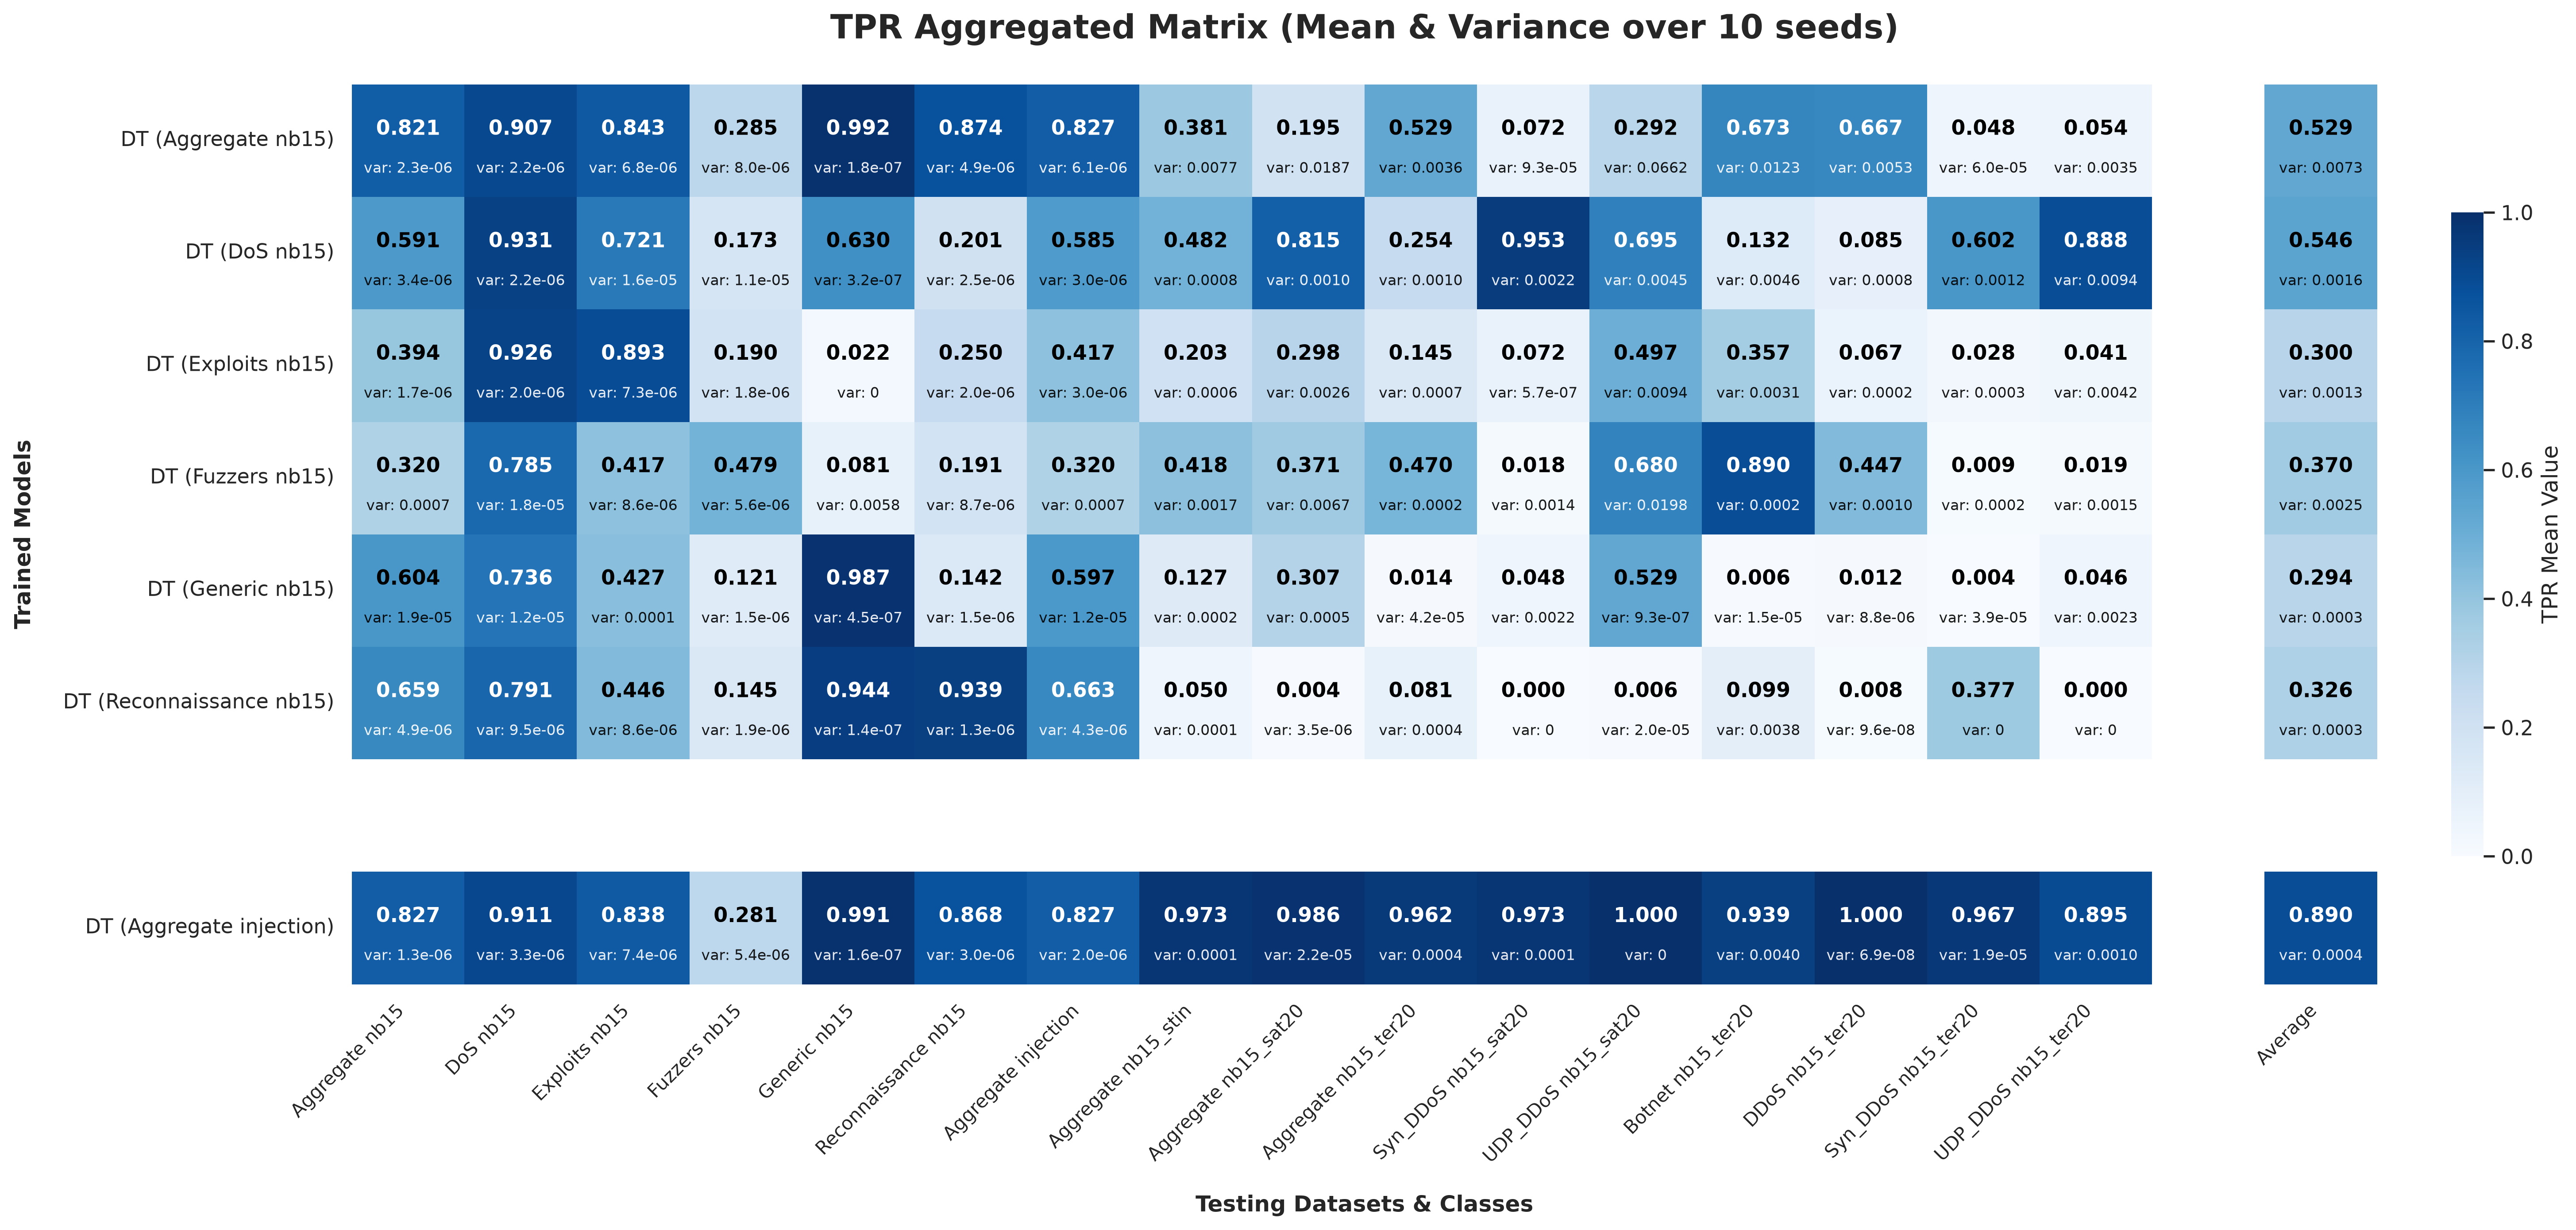
\includegraphics[
            width=\linewidth,
            height=0.80\textheight,
            keepaspectratio
        ] {images/chapter5/heatmaps/dt_TPR_aggregated_matrix_source_vs_baseline.png}
        \caption{Matrice aggregata della TPR per Decision Tree nel confronto tra modelli sorgente e baseline \texttt{INJECTION}. Per ciascuna cella sono riportate la media e la varianza calcolate sui $K=10$ seed.}
        \label{fig:heatmap_tpr_source_dt}
    \end{figure}
\end{landscape}

\begin{landscape}
    \begin{figure}[p]
        \centering

        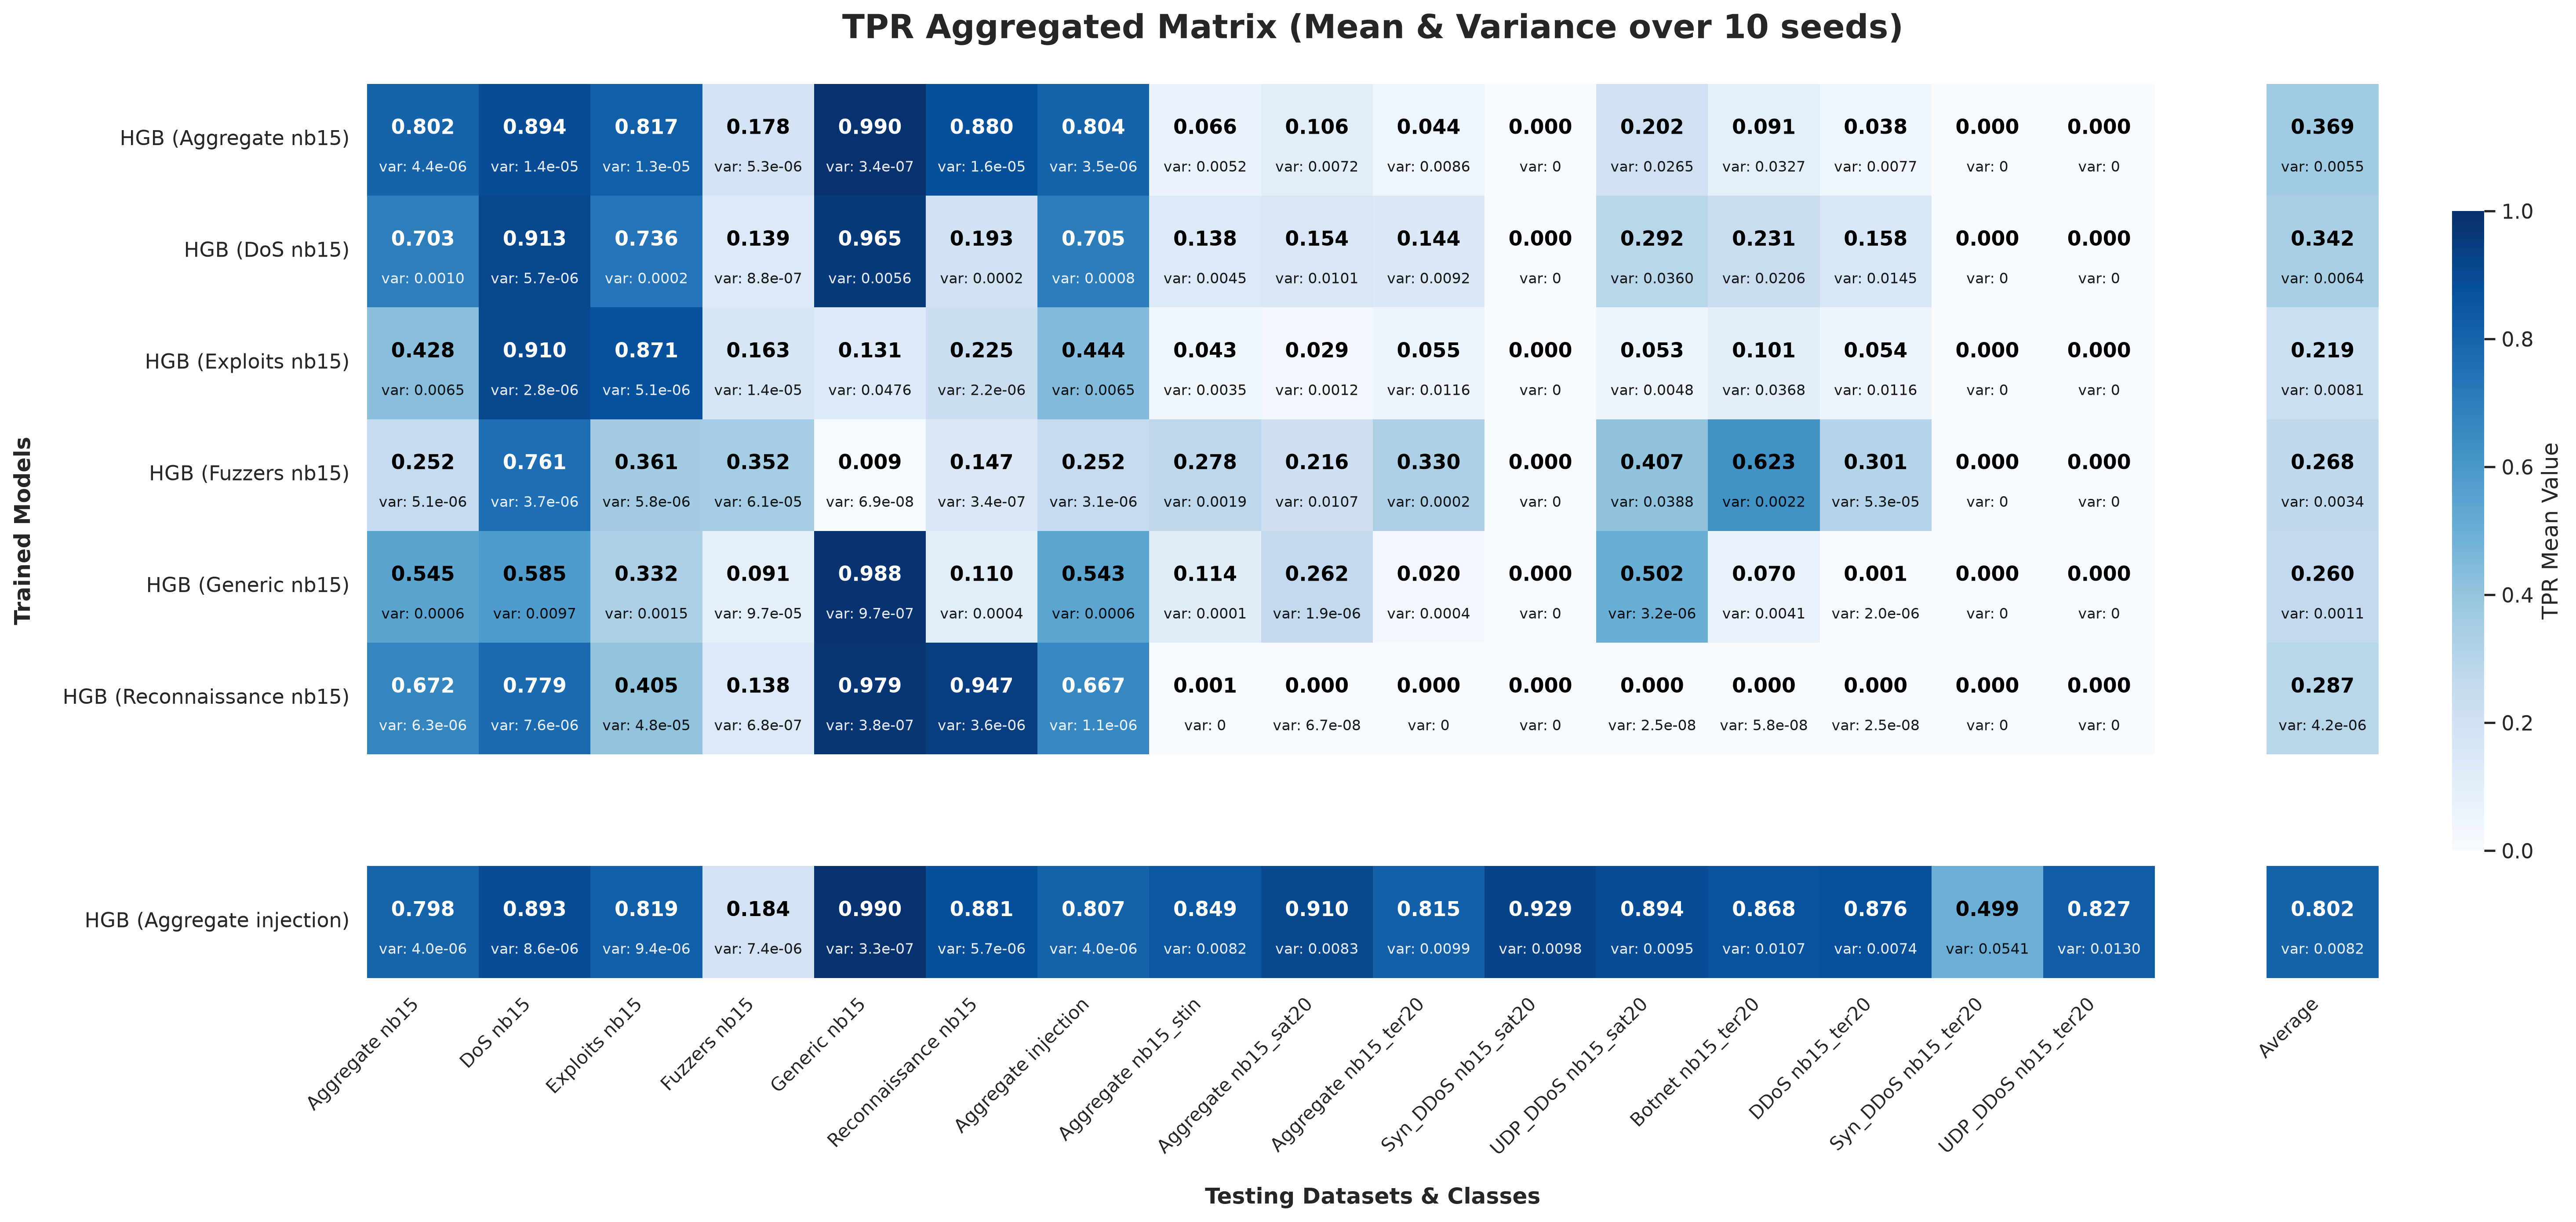
\includegraphics[
            width=\linewidth,
            height=0.80\textheight,
            keepaspectratio
        ] {images/chapter5/heatmaps/hgb_TPR_aggregated_matrix_source_vs_baseline.png}
        \caption{Matrice aggregata della TPR per Histogram-based Gradient Boosting nel confronto tra modelli sorgente e baseline \texttt{INJECTION}. Per ciascuna cella sono riportate la media e la varianza calcolate sui $K=10$ seed.}
        \label{fig:heatmap_tpr_source_hgb}
    \end{figure}
\end{landscape}

\begin{landscape}
    \begin{figure}[p]
        \centering

        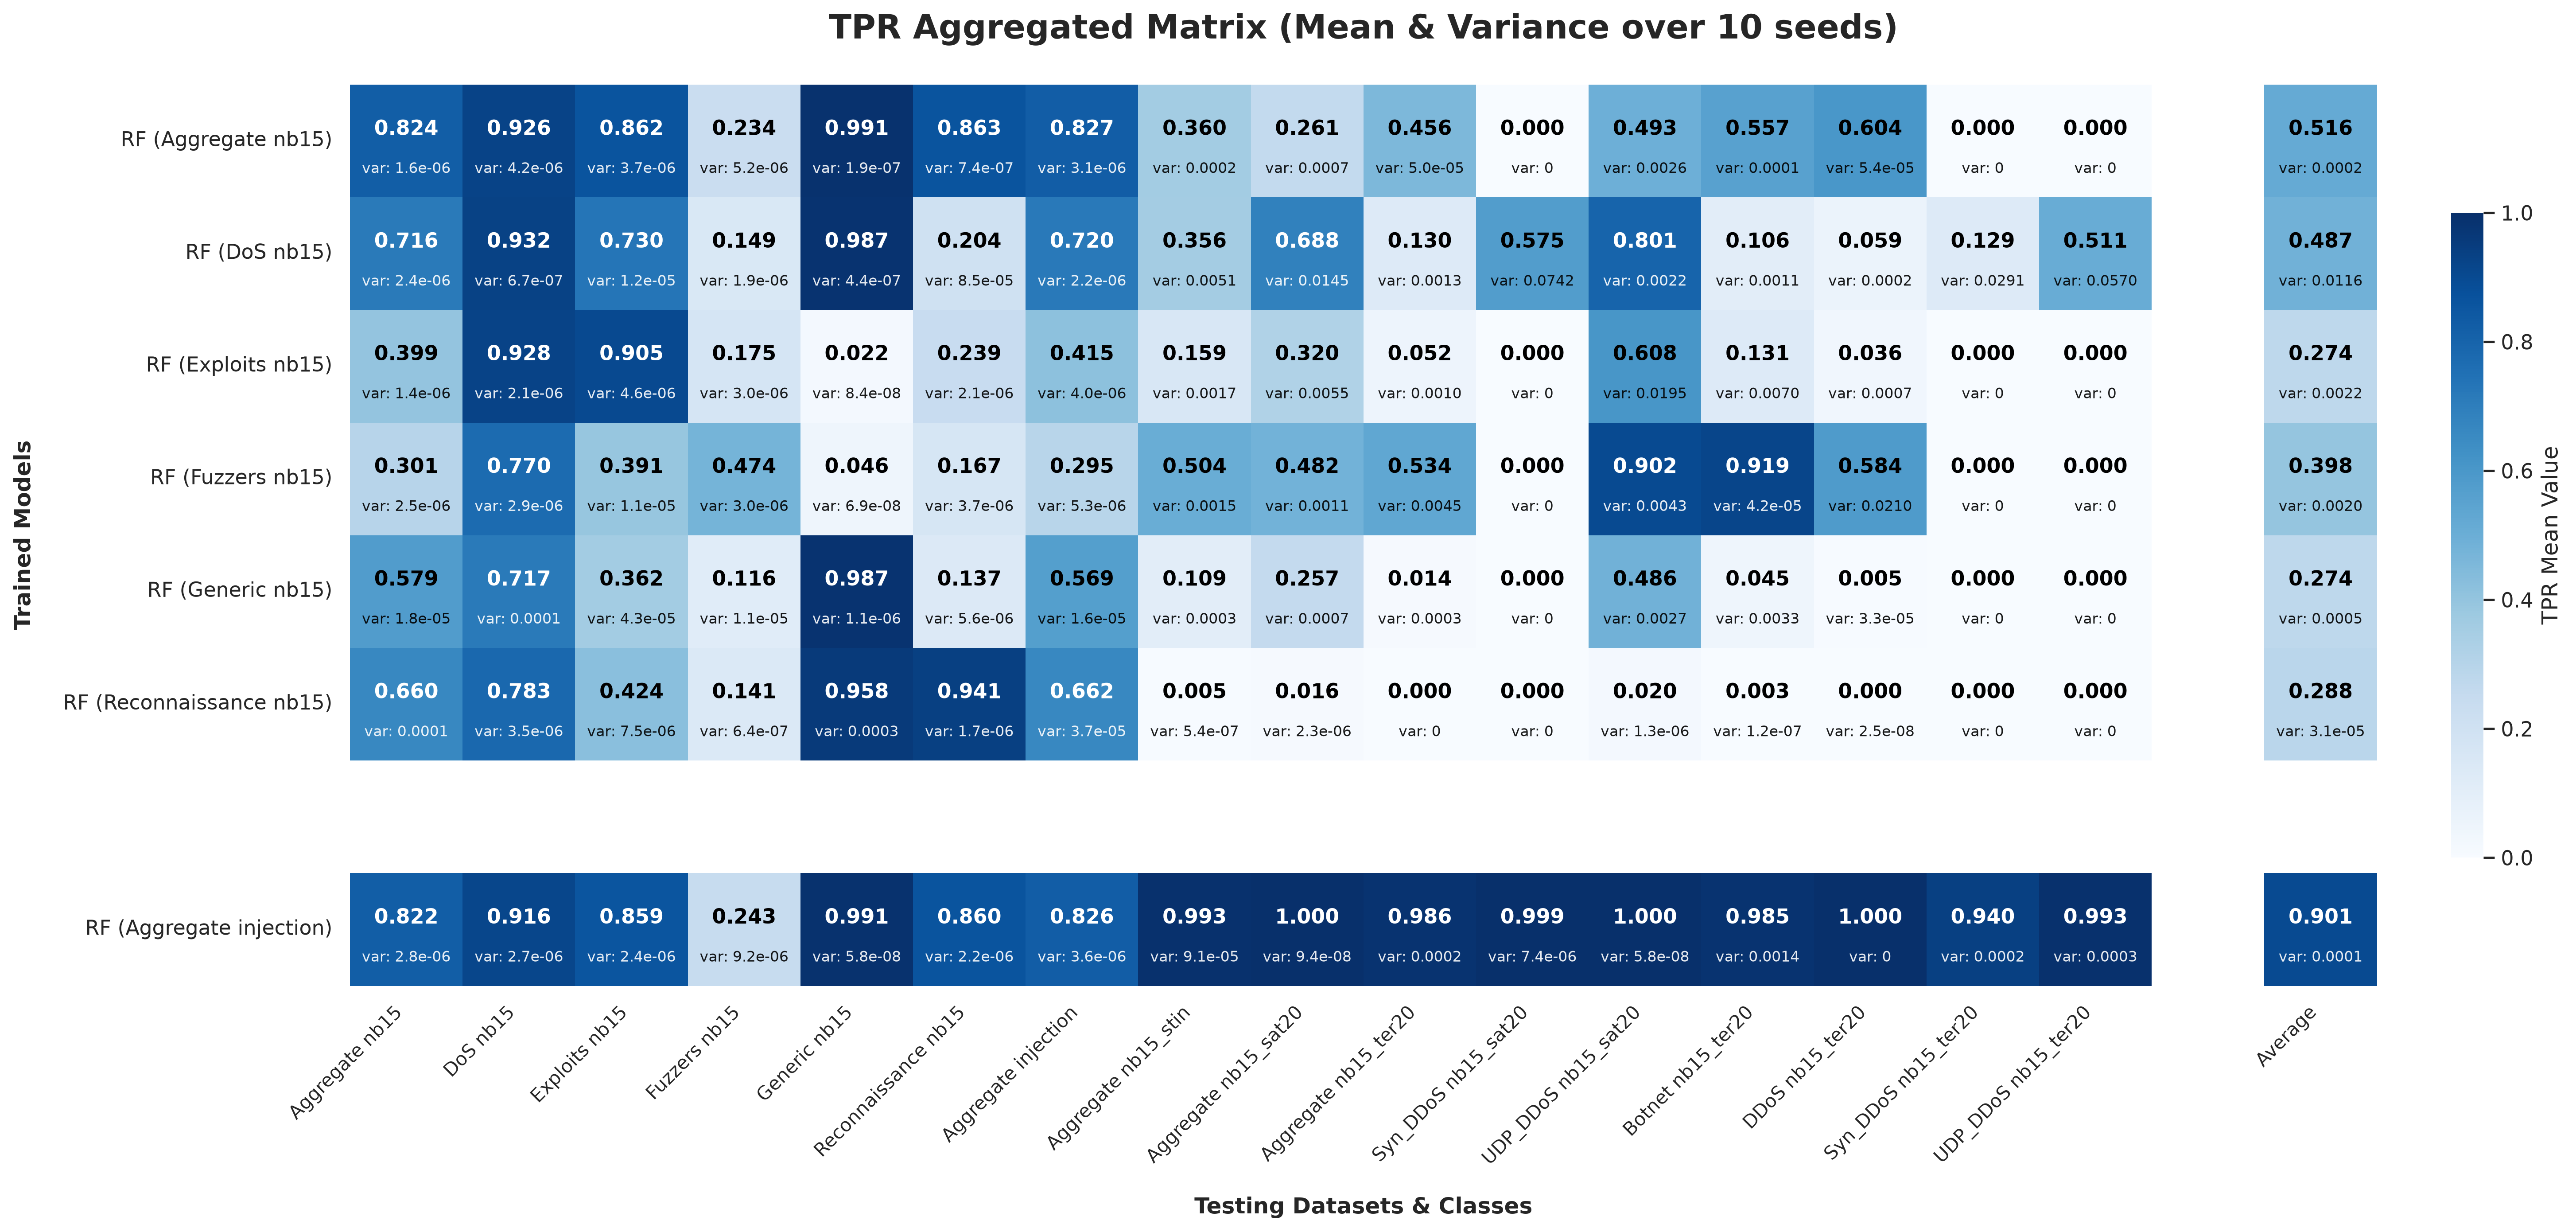
\includegraphics[
            width=\linewidth,
            height=0.80\textheight,
            keepaspectratio
        ] {images/chapter5/heatmaps/rf_TPR_aggregated_matrix_source_vs_baseline.png}
        \caption{Matrice aggregata della TPR per Random Forest nel confronto tra modelli sorgente e baseline \texttt{INJECTION}. Per ciascuna cella sono riportate la media e la varianza calcolate sui $K=10$ seed.}
        \label{fig:heatmap_tpr_source_rf}
    \end{figure}
\end{landscape}



% ==============================================================================
% MODELLI IBRIDI
% ==============================================================================

\section{Risultati Completi dei Modelli Ibridi}
\label{app:modelli_ibridi}

La presente sezione riporta il dettaglio numerico delle valutazioni dei modelli ibridi discusse nella Sezione~\ref{sec:risultati_modelli_ibridi}. 
Sono riportate separatamente le prestazioni sui benchmark target omologhi e i risultati della cross-evaluation sulle differenti distribuzioni considerate.

% ==============================================================================
% PRESTAZIONI OMOLOGHE DEI MODELLI IBRIDI
% ==============================================================================

\subsection{Prestazioni sui Benchmark Omologhi}

La Tabella~\ref{tab:ibridi_matched_seed42} riporta i valori di TPR e \textit{F1-Score} ottenuti dai modelli ibridi sui rispettivi benchmark target omologhi per il seed $s=42$.

\begin{table}[H]
    \centering
    \footnotesize
    \caption{TPR e F1-Score dei modelli ibridi sui rispettivi test set target omologhi per il seed $s=42$.}
    \label{tab:ibridi_matched_seed42}
    \begin{tabular}{lcc|cc|cc}
        \toprule
        & \multicolumn{2}{c|}{\textbf{DT}} & \multicolumn{2}{c|}{\textbf{HGB}} & \multicolumn{2}{c}{\textbf{RF}} \\
        \textbf{Modello / Test Set} & \textbf{TPR} & \textbf{F1} & \textbf{TPR} & \textbf{F1} & \textbf{TPR} & \textbf{F1} \\
        \midrule
        \texttt{nb15\_stin} (aggregato) & 0.9995 & 0.9997 & 0.9995 & 0.9997 & 0.9995 & 0.9997 \\
        \texttt{nb15\_sat20} (aggregato) & 0.9995 & 0.9997 & 0.9995 & 0.9997 & 0.9995 & 0.9997 \\
        \texttt{nb15\_ter20} (aggregato) & 1.0000 & 1.0000 & 1.0000 & 1.0000 & 1.0000 & 1.0000 \\
        \texttt{nb15\_sat20} (Syn\_DDoS) & 1.0000 & 1.0000 & 1.0000 & 1.0000 & 1.0000 & 1.0000 \\
        \texttt{nb15\_sat20} (UDP\_DDoS) & 1.0000 & 1.0000 & 1.0000 & 1.0000 & 1.0000 & 1.0000 \\
        \texttt{nb15\_ter20} (Botnet) & 1.0000 & 1.0000 & 1.0000 & 1.0000 & 1.0000 & 1.0000 \\
        \texttt{nb15\_ter20} (DDoS) & 1.0000 & 1.0000 & 1.0000 & 1.0000 & 1.0000 & 1.0000 \\
        \texttt{nb15\_ter20} (Syn\_DDoS) & 1.0000 & 1.0000 & 1.0000 & 1.0000 & 1.0000 & 1.0000 \\
        \texttt{nb15\_ter20} (UDP\_DDoS) & 1.0000 & 1.0000 & 1.0000 & 1.0000 & 1.0000 & 1.0000 \\
        \bottomrule
    \end{tabular}
\end{table}


% ==============================================================================
% CROSS-EVALUATION DEI MODELLI IBRIDI
% ==============================================================================

\subsection{Cross-Evaluation dei Modelli Ibridi}

La Tabella~\ref{tab:ibridi_domain_transfer_tpr} sintetizza la TPR media multi-seed dei modelli ibridi nella cross-evaluation sui benchmark sorgente, sulla configurazione \texttt{INJECTION} e sui benchmark target.

\begin{table}[H]
    \centering
    \footnotesize
    \caption{TPR media multi-seed dei modelli ibridi sui benchmark sorgente, \texttt{INJECTION} e target. Le colonne NB15 e Target rappresentano rispettivamente la media sui sei e sui nove test set dei corrispondenti gruppi.}
    \label{tab:ibridi_domain_transfer_tpr}
    \resizebox{\textwidth}{!}{
    \begin{tabular}{lccc|ccc|ccc}
        \toprule
        & \multicolumn{3}{c|}{\textbf{DT}} & \multicolumn{3}{c|}{\textbf{HGB}} & \multicolumn{3}{c}{\textbf{RF}} \\
        \textbf{Modello} & \textbf{NB15} & \textbf{INJ.} & \textbf{Target} & \textbf{NB15} & \textbf{INJ.} & \textbf{Target} & \textbf{NB15} & \textbf{INJ.} & \textbf{Target} \\
        \midrule
        \texttt{nb15\_stin\_aggregate} & 0.000000 & 0.00320 & 0.999922 & 0.000000 & 0.00320 & 0.999944 & 0.000000 & 0.00320 & 0.999922 \\
        \texttt{nb15\_sat20\_aggregate} & 0.000000 & 0.00320 & 0.999889 & 0.000000 & 0.00320 & 0.981796 & 0.000000 & 0.00320 & 0.999894 \\
        \texttt{nb15\_ter20\_aggregate} & 0.000000 & 0.00320 & 0.999922 & 0.000000 & 0.00320 & 0.999944 & 0.000000 & 0.00320 & 0.999906 \\
        \texttt{nb15\_sat20\_syn\_ddos} & 0.000000 & 0.00050 & 0.424387 & 0.000000 & 0.00050 & 0.315589 & 0.000000 & 0.00050 & 0.443831 \\
        \texttt{nb15\_sat20\_udp\_ddos} & 0.000000 & 0.00320 & 0.974900 & 0.000000 & 0.00270 & 0.551311 & 0.000000 & 0.00320 & 0.898881 \\
        \texttt{nb15\_ter20\_botnet} & 0.000000 & 0.00320 & 0.952424 & 0.000000 & 0.00310 & 0.842102 & 0.000000 & 0.00320 & 0.910777 \\
        \texttt{nb15\_ter20\_ddos} & 0.000000 & 0.00310 & 0.829924 & 0.000000 & 0.00270 & 0.551311 & 0.000000 & 0.00285 & 0.664007 \\
        \texttt{nb15\_ter20\_syn\_ddos} & 0.000000 & 0.00320 & 0.999928 & 0.000025 & 0.00196 & 0.629574 & 0.000000 & 0.00320 & 0.999910 \\
        \texttt{nb15\_ter20\_udp\_ddos} & 0.000000 & 0.00320 & 0.978669 & 0.000000 & 0.00050 & 0.350036 & 0.000000 & 0.00050 & 0.448567 \\
        \bottomrule
    \end{tabular}
    }
\end{table}


% ==============================================================================
% HEATMAP TPR AGGREGATE -- MODELLI IBRIDI VS BASELINE
% ==============================================================================

\subsection{Mappe di Calore Aggregate della TPR}
\label{app:heatmap_tpr_ibridi}

Le Figure~\ref{fig:heatmap_tpr_hybrid_dt}, \ref{fig:heatmap_tpr_hybrid_hgb} e \ref{fig:heatmap_tpr_hybrid_rf} completano la caratterizzazione della \textit{cross-evaluation} dei modelli ibridi mediante una rappresentazione grafica delle matrici aggregate della TPR.

Le righe comprendono i modelli aggregati e biclasse addestrati utilizzando la componente malevola target, mentre le colonne corrispondono ai medesimi benchmark sorgente, \texttt{INJECTION} e target impiegati nel protocollo di valutazione. 
La baseline \texttt{INJECTION} è riportata separatamente come riferimento comune. 
Analogamente alle matrici relative ai modelli sorgente, ciascuna cella riporta la TPR media e la relativa varianza ottenute sui $K=10$ seed, mentre la colonna finale sintetizza la risposta media lungo l'intera matrice di valutazione.

Tale rappresentazione integra il dettaglio numerico della Tabella~\ref{tab:ibridi_domain_transfer_tpr}, consentendo di preservare nell'appendice la struttura completa dei risultati multi-seed senza appesantire la discussione principale del Capitolo~\ref{ch:risultati}.

\begin{landscape}
    \begin{figure}[p]
        \centering

        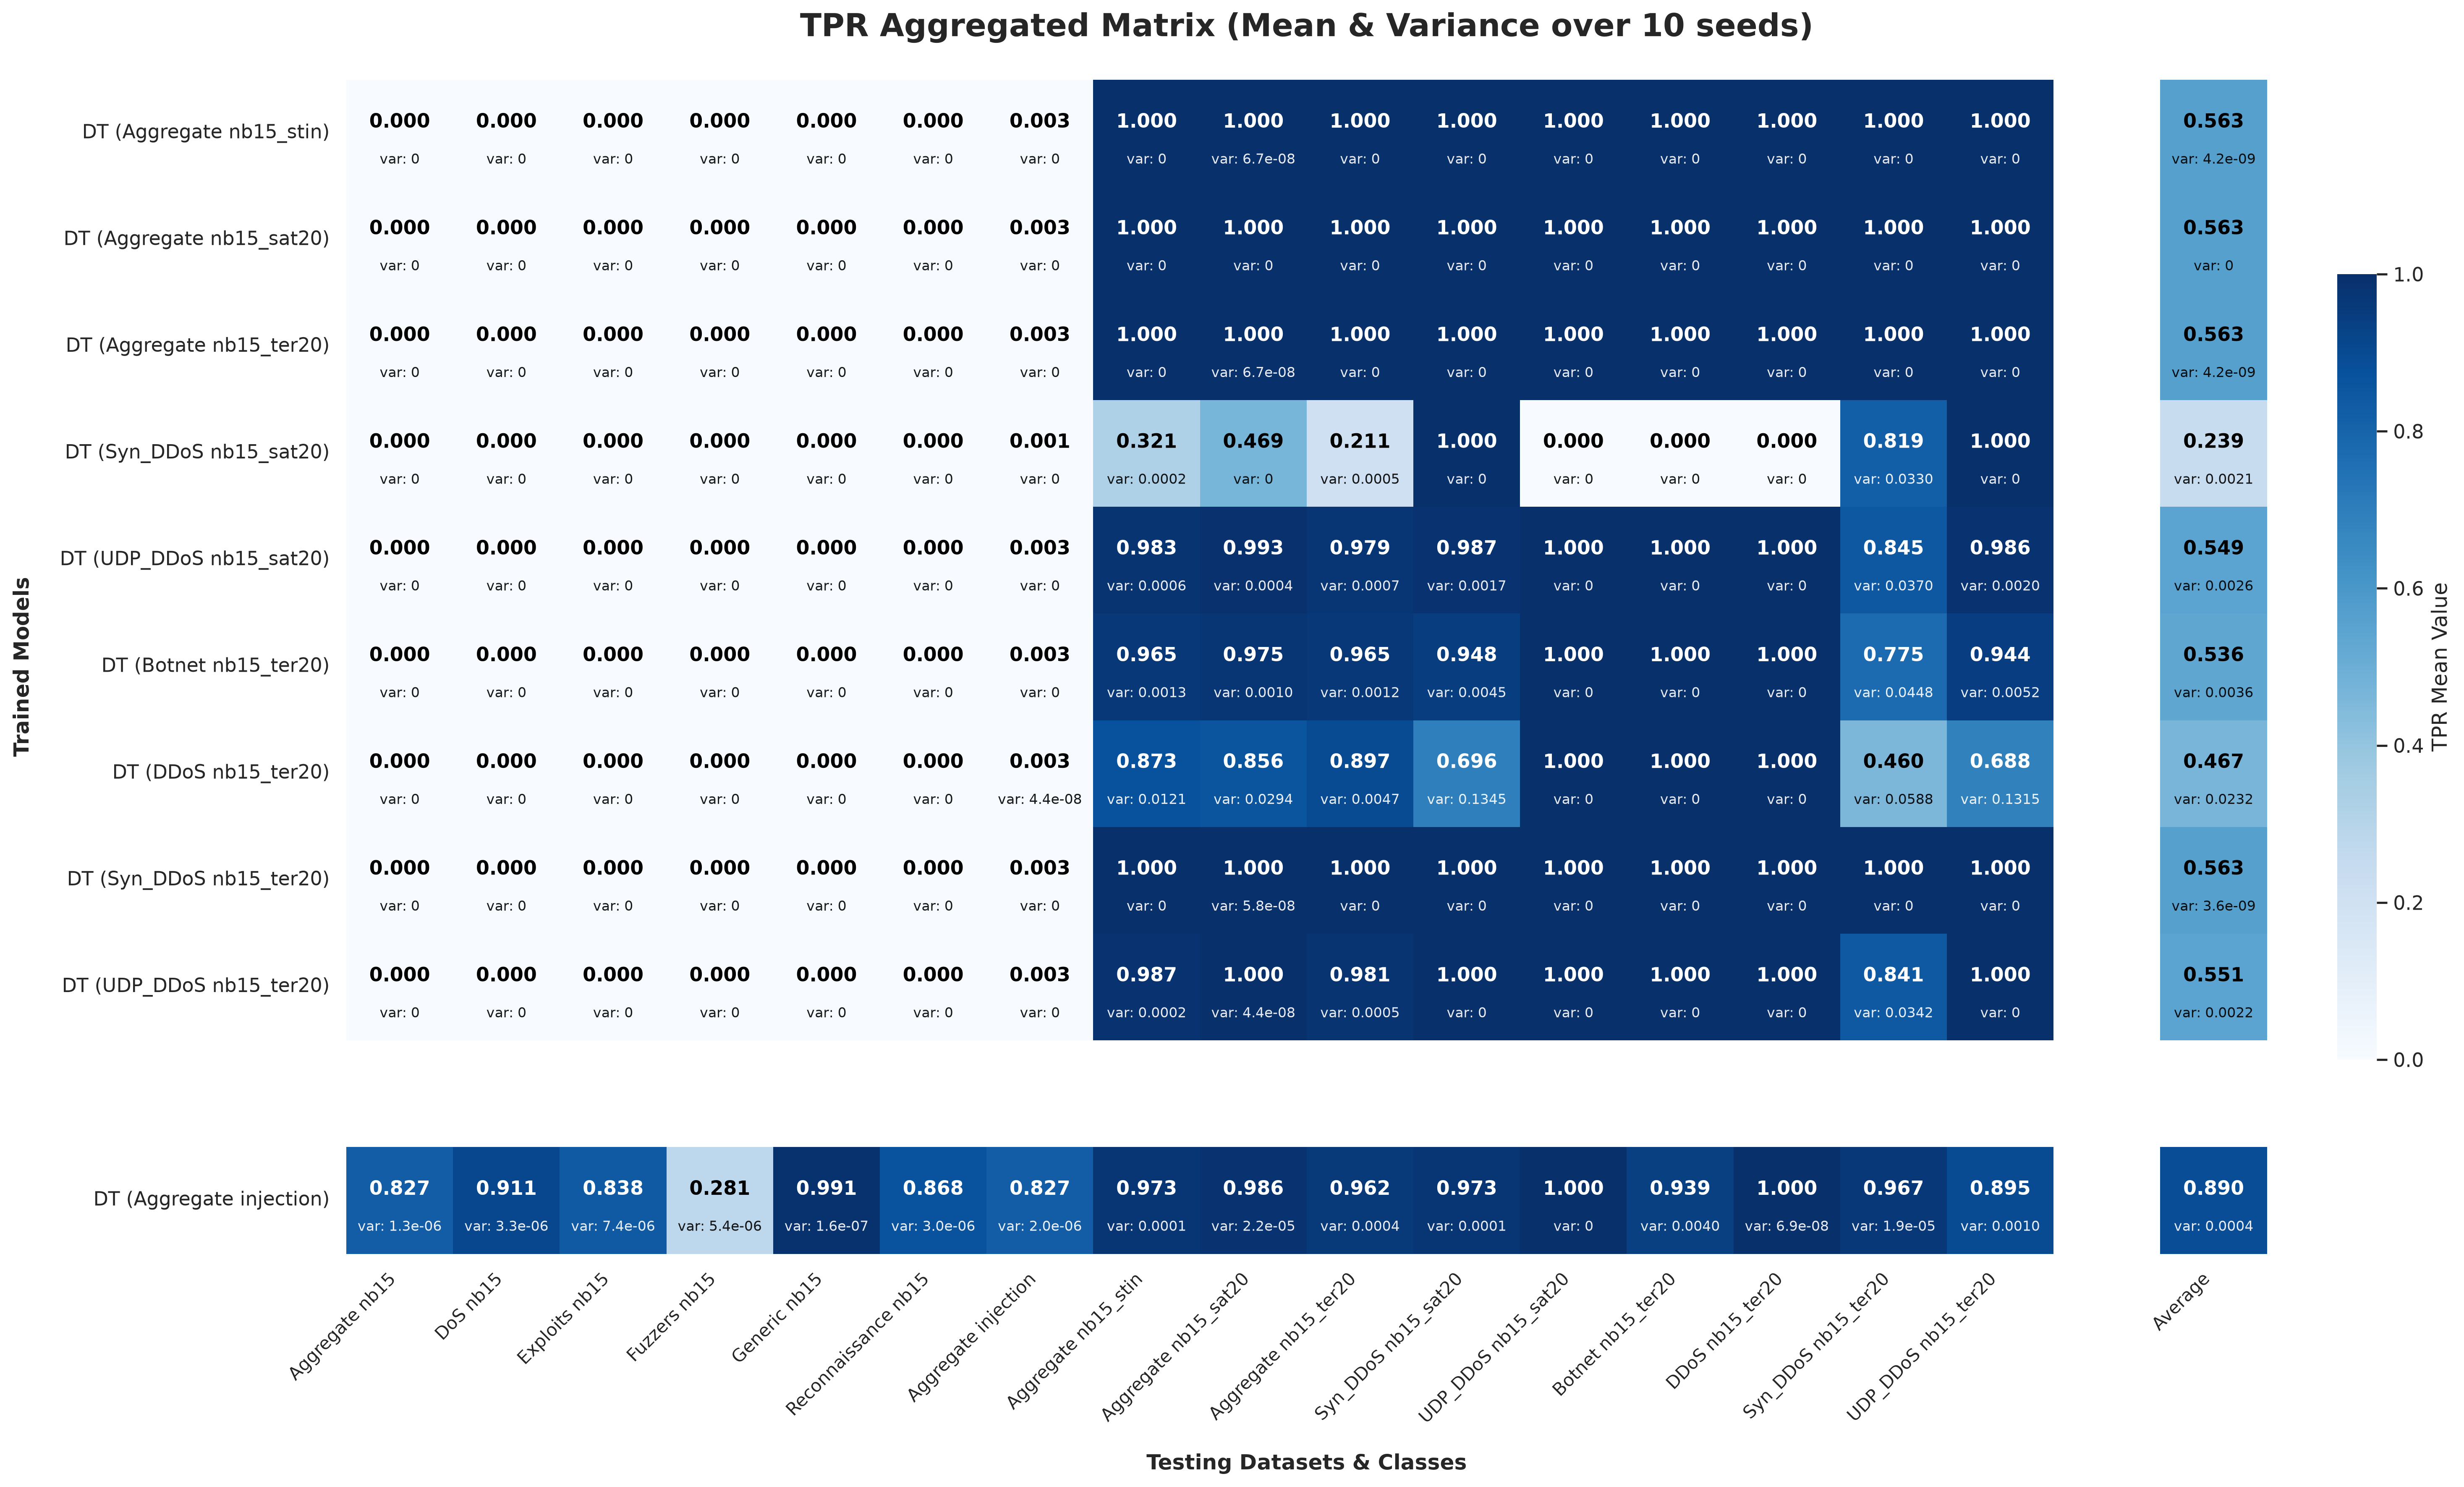
\includegraphics[
            width=\linewidth,
            height=0.80\textheight,
            keepaspectratio
        ] {images/chapter5/heatmaps/dt_TPR_aggregated_matrix_hybrid_vs_baseline.png}
        \caption{Matrice aggregata della TPR per Decision Tree nel confronto tra modelli ibridi e baseline \texttt{INJECTION}. Per ciascuna cella sono riportate la media e la varianza calcolate sui $K=10$ seed.}
        \label{fig:heatmap_tpr_hybrid_dt}
    \end{figure}
\end{landscape}

\begin{landscape}
    \begin{figure}[p]
        \centering

        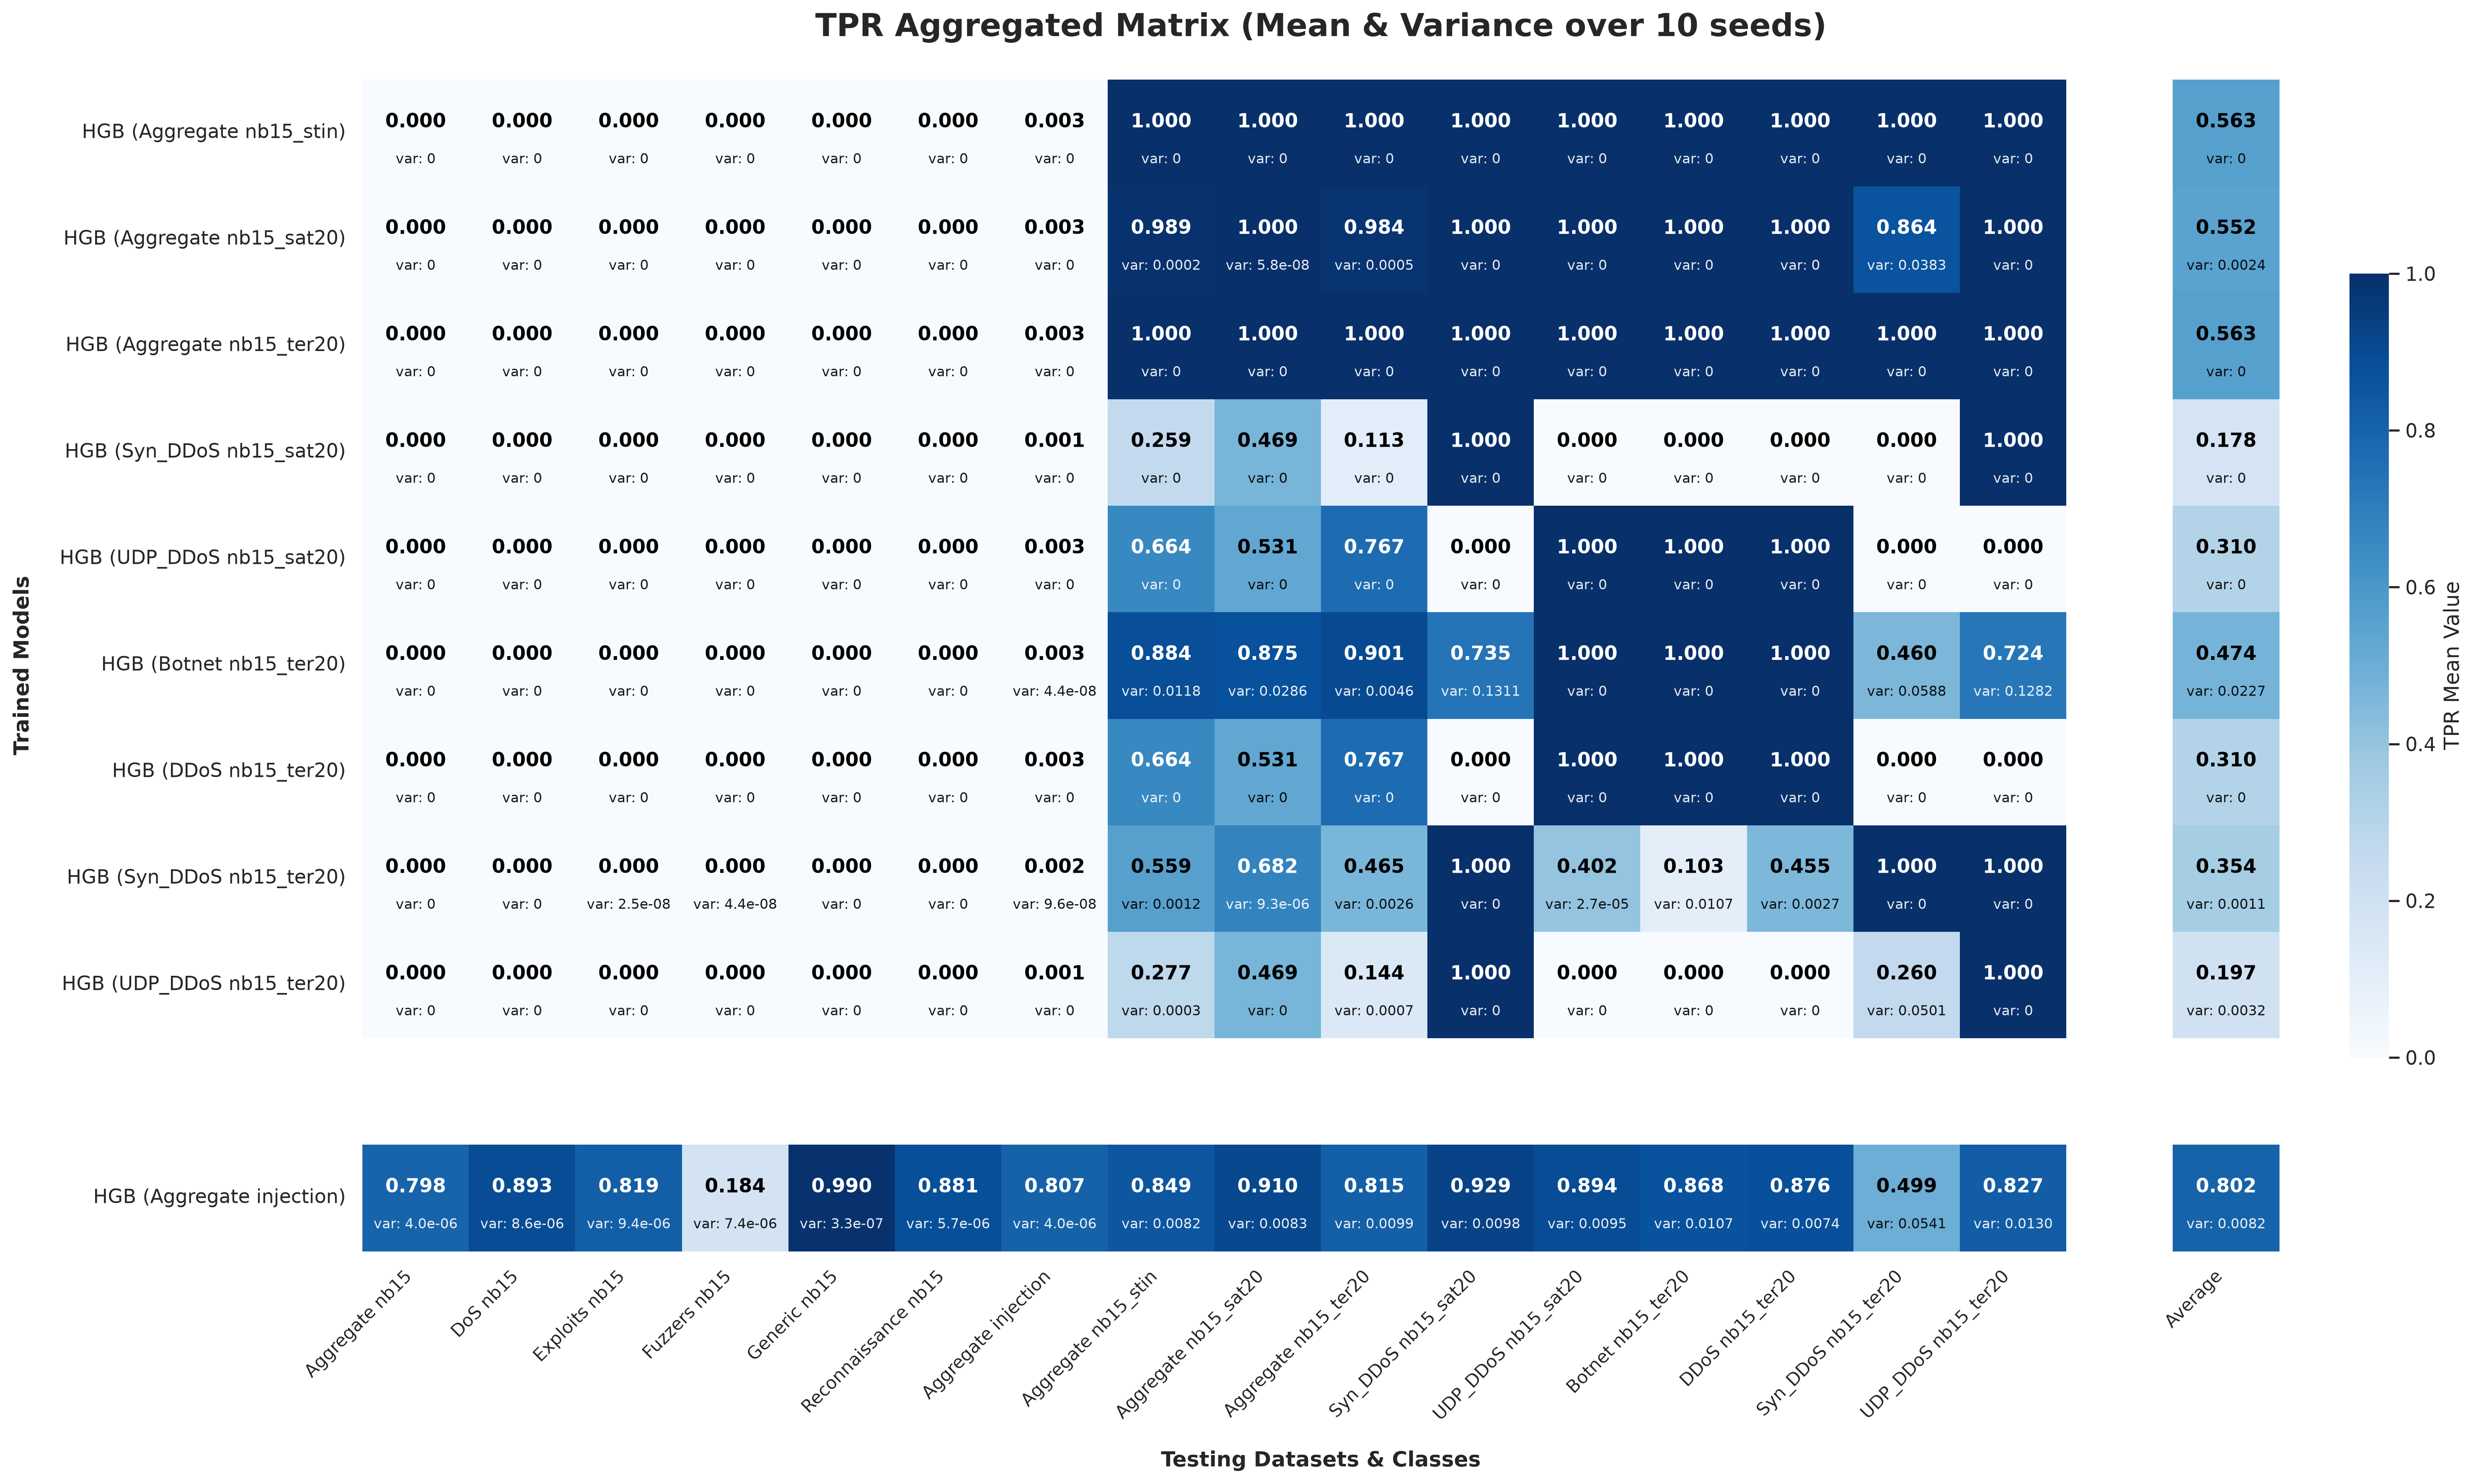
\includegraphics[
            width=\linewidth,
            height=0.80\textheight,
            keepaspectratio
        ] {images/chapter5/heatmaps/hgb_TPR_aggregated_matrix_hybrid_vs_baseline.png}
        \caption{Matrice aggregata della TPR per Histogram-based Gradient Boosting nel confronto tra modelli ibridi e baseline \texttt{INJECTION}. Per ciascuna cella sono riportate la media e la varianza calcolate sui $K=10$ seed.}
        \label{fig:heatmap_tpr_hybrid_hgb}
    \end{figure}
\end{landscape}

\begin{landscape}
    \begin{figure}[p]
        \centering

        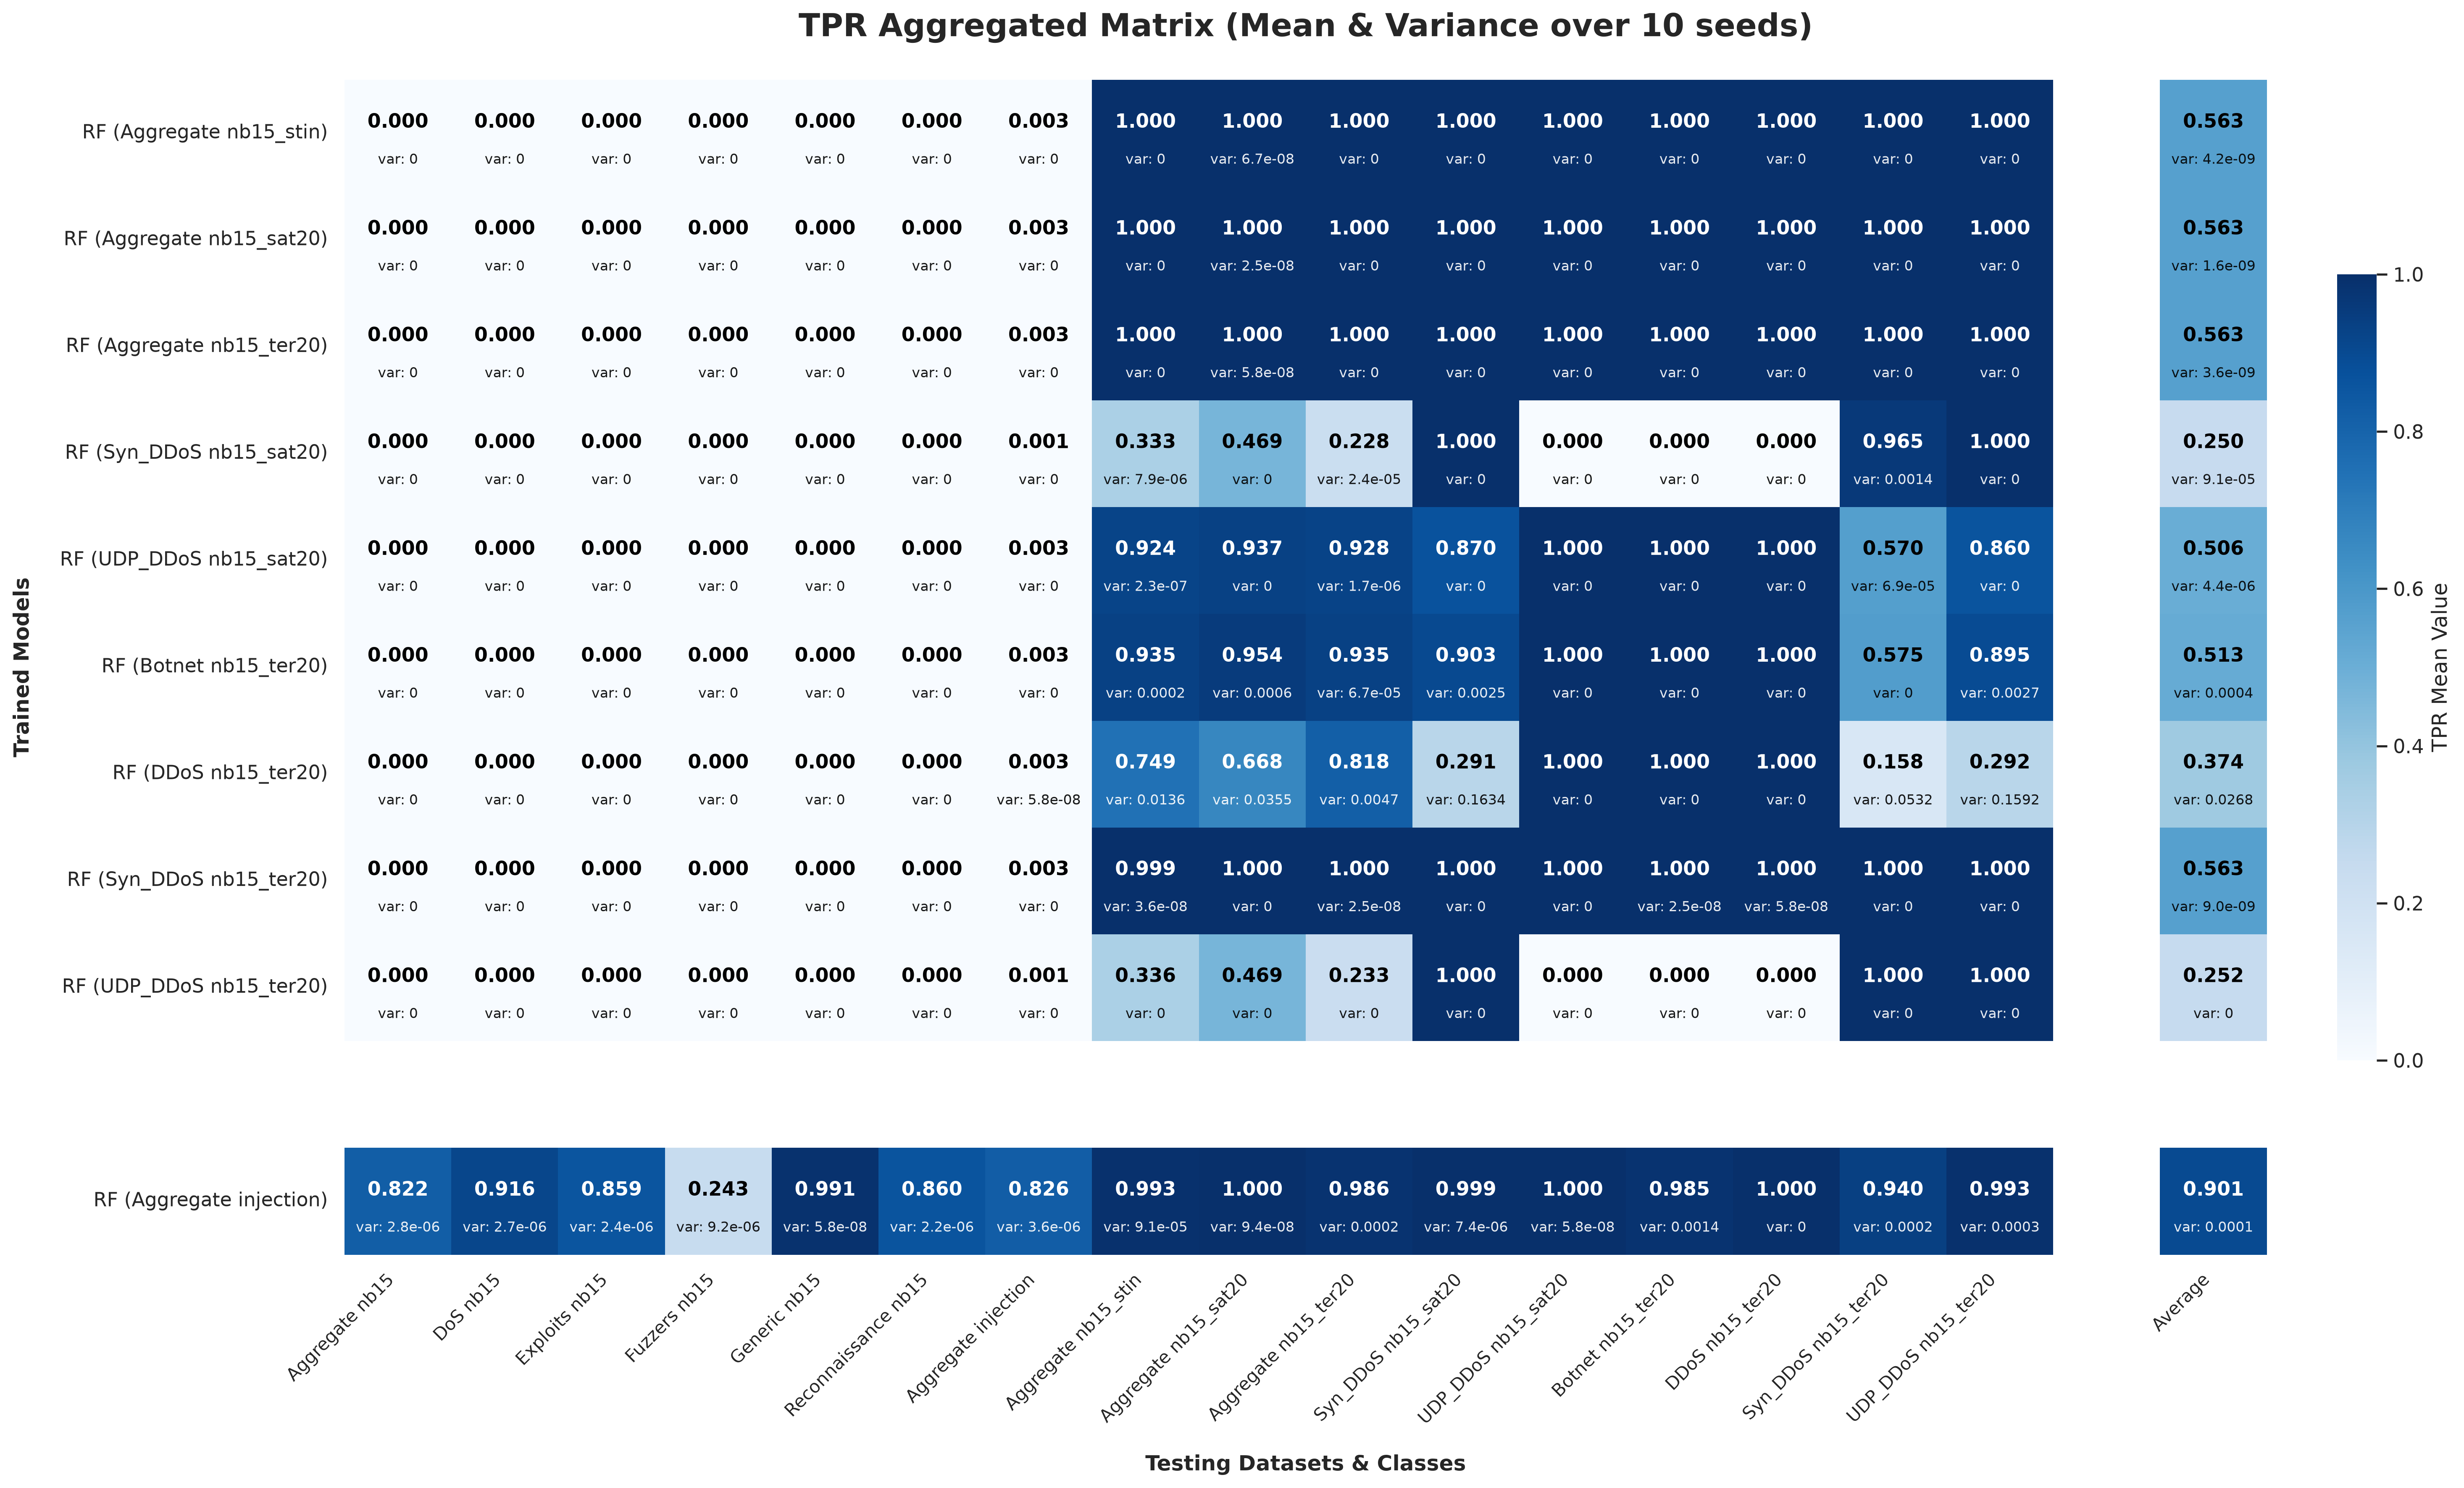
\includegraphics[
            width=\linewidth,
            height=0.80\textheight,
            keepaspectratio
        ] {images/chapter5/heatmaps/rf_TPR_aggregated_matrix_hybrid_vs_baseline.png}
        \caption{Matrice aggregata della TPR per Random Forest nel confronto tra modelli ibridi e baseline \texttt{INJECTION}. Per ciascuna cella sono riportate la media e la varianza calcolate sui $K=10$ seed.}
        \label{fig:heatmap_tpr_hybrid_rf}
    \end{figure}
\end{landscape}



% ==============================================================================
% ANALISI STATISTICA
% ==============================================================================

\section{Risultati Completi dei Test Statistici}
\label{app:welch}

La presente sezione raccoglie le statistiche descrittive e i risultati completi dei test $t$ di Welch discussi nel Capitolo~\ref{ch:risultati}. 
I confronti sono organizzati separatamente per i modelli sorgente e per i modelli ibridi, assumendo in entrambi i casi la configurazione \texttt{INJECTION} come riferimento sperimentale.

% ==============================================================================
% TEST DI WELCH -- MODELLI SORGENTE
% ==============================================================================

\subsection{Modelli Sorgente rispetto alla Baseline INJECTION}

Prima dell'applicazione del test inferenziale, la Tabella~\ref{tab:sorgente_welch_descriptive} riporta le statistiche descrittive dei valori medi di \textit{F1-Score} ottenuti sui $10$ seed dalla baseline \texttt{INJECTION} e dai modelli sorgente.

\begin{table}[H]
    \centering
    \footnotesize
    \caption{Media e deviazione standard campionaria dei valori $\overline{F1}_{i}^{(k)}$ sui $10$ seed per la baseline e i modelli sorgente. $\Delta F1$ è calcolato come baseline meno modello sorgente.}
    \label{tab:sorgente_welch_descriptive}
    \resizebox{\textwidth}{!}{
    \begin{tabular}{lccc|ccc|ccc}
        \toprule
        \multirow{2}{*}{\textbf{Modello}} & \multicolumn{3}{c|}{\textbf{DT}} & \multicolumn{3}{c|}{\textbf{HGB}} & \multicolumn{3}{c}{\textbf{RF}} \\
        & $\boldsymbol{\overline{\overline{F1}}}$ & $\boldsymbol{s}$ & $\boldsymbol{\Delta F1}$ & $\boldsymbol{\overline{\overline{F1}}}$ & $\boldsymbol{s}$ & $\boldsymbol{\Delta F1}$ & $\boldsymbol{\overline{\overline{F1}}}$ & $\boldsymbol{s}$ & $\boldsymbol{\Delta F1}$ \\
        \midrule
        \texttt{injection\_aggregate} & 0.86039 & 0.00352 & -- & 0.85407 & 0.03634 & -- & 0.89022 & 0.00245 & -- \\
        \texttt{nb15\_aggregate} & 0.56308 & 0.04017 & $+0.29731$ & 0.41231 & 0.05289 & $+0.44177$ & 0.57651 & 0.00647 & $+0.31371$ \\
        \texttt{nb15\_dos} & 0.63163 & 0.01413 & $+0.22876$ & 0.41671 & 0.05056 & $+0.43737$ & 0.57207 & 0.05750 & $+0.31815$ \\
        \texttt{nb15\_exploits} & 0.37742 & 0.01922 & $+0.48297$ & 0.27167 & 0.03931 & $+0.58240$ & 0.34199 & 0.02338 & $+0.54823$ \\
        \texttt{nb15\_fuzzers} & 0.38778 & 0.02178 & $+0.47261$ & 0.35018 & 0.02762 & $+0.50390$ & 0.41666 & 0.01181 & $+0.47356$ \\
        \texttt{nb15\_generic} & 0.37596 & 0.01366 & $+0.48443$ & 0.33977 & 0.01613 & $+0.51430$ & 0.35185 & 0.01199 & $+0.53837$ \\
        \texttt{nb15\_reconnaissance} & 0.38165 & 0.00983 & $+0.47874$ & 0.32058 & 0.00053 & $+0.53349$ & 0.32659 & 0.00129 & $+0.56364$ \\
        \bottomrule
    \end{tabular}
    }
\end{table}

Sulla base dei campioni così caratterizzati, la Tabella~\ref{tab:sorgente_welch_results} riporta, per ciascun modello sorgente e classificatore, la statistica $t$, il corrispondente $p$-value e l'esito della verifica di significatività rispetto alla soglia $\alpha=0{,}05$.

\begin{table}[H]
    \centering
    \footnotesize
    \caption{Risultati del test $t$ di Welch tra \texttt{injection\_aggregate} e i modelli sorgente, con $\alpha=0{,}05$.}
    \label{tab:sorgente_welch_results}
    \resizebox{\textwidth}{!}{
    \begin{tabular}{lccc|ccc|ccc}
        \toprule
        \multirow{2}{*}{\textbf{Modello confrontato}} & \multicolumn{3}{c|}{\textbf{DT}} & \multicolumn{3}{c|}{\textbf{HGB}} & \multicolumn{3}{c}{\textbf{RF}} \\
        & $\boldsymbol{t}$ & $\boldsymbol{p}$ & \textbf{Sign.} & $\boldsymbol{t}$ & $\boldsymbol{p}$ & \textbf{Sign.} & $\boldsymbol{t}$ & $\boldsymbol{p}$ & \textbf{Sign.} \\
        \midrule
        \texttt{nb15\_aggregate} & 23.3150 & $1.8720\times10^{-9}$ & Sì & 21.7698 & $2.7489\times10^{-13}$ & Sì & 143.4423 & $4.0594\times10^{-20}$ & Sì \\
        \texttt{nb15\_dos} & 49.6699 & $2.0529\times10^{-13}$ & Sì & 22.2139 & $1.2228\times10^{-13}$ & Sì & 17.4802 & $2.8399\times10^{-8}$ & Sì \\
        \texttt{nb15\_exploits} & 78.1496 & $8.6609\times10^{-15}$ & Sì & 34.4010 & $8.5047\times10^{-18}$ & Sì & 73.7488 & $4.5473\times10^{-14}$ & Sì \\
        \texttt{nb15\_fuzzers} & 67.7344 & $4.8440\times10^{-14}$ & Sì & 34.9112 & $4.0724\times10^{-17}$ & Sì & 124.1469 & $5.8434\times10^{-17}$ & Sì \\
        \texttt{nb15\_generic} & 108.6316 & $6.0030\times10^{-17}$ & Sì & 40.9031 & $1.2819\times10^{-14}$ & Sì & 139.1262 & $2.0720\times10^{-17}$ & Sì \\
        \texttt{nb15\_reconnaissance} & 144.9748 & $8.7646\times10^{-20}$ & Sì & 46.4184 & $4.9595\times10^{-12}$ & Sì & 643.0892 & $5.6491\times10^{-32}$ & Sì \\
        \bottomrule
    \end{tabular}
    }
\end{table}


\subsection{Modelli Ibridi rispetto alla Baseline INJECTION}

Analogamente al confronto precedente, la Tabella~\ref{tab:ibridi_welch_descriptive} riporta le statistiche descrittive dei valori medi di \textit{F1-Score} ottenuti sui $10$ seed dalla baseline \texttt{INJECTION} e dalle differenti configurazioni dei modelli ibridi.

\begin{table}[H]
    \centering
    \footnotesize
    \caption{Media e deviazione standard campionaria dei valori medi di F1-Score sui $10$ seed per la baseline e i modelli ibridi. $\Delta F1$ è calcolato come baseline meno modello ibrido.}
    \label{tab:ibridi_welch_descriptive}
    \resizebox{\textwidth}{!}{
    \begin{tabular}{lccc|ccc|ccc}
        \toprule
        \multirow{2}{*}{\textbf{Modello}} & \multicolumn{3}{c|}{\textbf{DT}} & \multicolumn{3}{c|}{\textbf{HGB}} & \multicolumn{3}{c}{\textbf{RF}} \\
         & $\boldsymbol{\overline{\overline{F1}}}$ & $\boldsymbol{s}$ & $\boldsymbol{\Delta F1}$ & $\boldsymbol{\overline{\overline{F1}}}$ & $\boldsymbol{s}$ & $\boldsymbol{\Delta F1}$ & $\boldsymbol{\overline{\overline{F1}}}$ & $\boldsymbol{s}$ & $\boldsymbol{\Delta F1}$ \\
        \midrule
        \texttt{injection\_aggregate} & 0.860388 & 0.003516 & -- & 0.854074 & 0.036341 & -- & 0.890221 & 0.002452 & -- \\
        \texttt{nb15\_sat20\_aggregate} & 0.562863 & 0.000000 & $+0.297526$ & 0.556714 & 0.009015 & $+0.297360$ & 0.562864 & 0.000006 & $+0.327357$ \\
        \texttt{nb15\_sat20\_syn\_ddos} & 0.272674 & 0.010401 & $+0.587714$ & 0.203331 & 0.000000 & $+0.650743$ & 0.280766 & 0.001831 & $+0.609456$ \\
        \texttt{nb15\_sat20\_udp\_ddos} & 0.554609 & 0.011598 & $+0.305779$ & 0.335325 & 0.000000 & $+0.518749$ & 0.529931 & 0.000483 & $+0.360290$ \\
        \texttt{nb15\_stin\_aggregate} & 0.562874 & 0.000010 & $+0.297514$ & 0.562881 & 0.000000 & $+0.291193$ & 0.562874 & 0.000010 & $+0.327348$ \\
        \texttt{nb15\_ter20\_aggregate} & 0.562874 & 0.000010 & $+0.297514$ & 0.562881 & 0.000000 & $+0.291193$ & 0.562868 & 0.000009 & $+0.327353$ \\
        \texttt{nb15\_ter20\_botnet} & 0.547373 & 0.015805 & $+0.313016$ & 0.496752 & 0.078046 & $+0.357322$ & 0.533624 & 0.005028 & $+0.356598$ \\
        \texttt{nb15\_ter20\_ddos} & 0.491250 & 0.082180 & $+0.369138$ & 0.335325 & 0.000000 & $+0.518749$ & 0.401911 & 0.085435 & $+0.488310$ \\
        \texttt{nb15\_ter20\_syn\_ddos} & 0.562876 & 0.000009 & $+0.297513$ & 0.408438 & 0.018932 & $+0.445636$ & 0.562871 & 0.000022 & $+0.327351$ \\
        \texttt{nb15\_ter20\_udp\_ddos} & 0.555778 & 0.008641 & $+0.304611$ & 0.230466 & 0.023354 & $+0.623608$ & 0.282475 & 0.000000 & $+0.607746$ \\
        \bottomrule
    \end{tabular}
    }
\end{table}

La Tabella~\ref{tab:ibridi_welch_results} completa l'analisi inferenziale riportando, per ciascun modello ibrido e classificatore, la statistica $t$, il corrispondente $p$-value e l'esito della verifica di significatività rispetto alla soglia $\alpha=0{,}05$.

\begin{table}[H]
    \centering
    \footnotesize
    \caption{Risultati del test $t$ di Welch tra \texttt{injection\_aggregate} e i modelli ibridi, con $\alpha=0{,}05$.}
    \label{tab:ibridi_welch_results}
    \resizebox{\textwidth}{!}{
    \begin{tabular}{lccc|ccc|ccc}
        \toprule
        \multirow{2}{*}{\textbf{Modello confrontato}} & \multicolumn{3}{c|}{\textbf{DT}} & \multicolumn{3}{c|}{\textbf{HGB}} & \multicolumn{3}{c}{\textbf{RF}} \\
        & $\boldsymbol{t}$ & $\boldsymbol{p}$ & \textbf{Sign.} & $\boldsymbol{t}$ & $\boldsymbol{p}$ & \textbf{Sign.} & $\boldsymbol{t}$ & $\boldsymbol{p}$ & \textbf{Sign.} \\
        \midrule
        \texttt{nb15\_sat20\_aggregate} & 267.5863 & $7.2356\times10^{-19}$ & Sì & 25.1143 & $1.9370\times10^{-10}$ & Sì & 422.2333 & $1.1929\times10^{-20}$ & Sì \\
        \texttt{nb15\_sat20\_syn\_ddos} & 169.2801 & $3.4456\times10^{-20}$ & Sì & 56.6262 & $8.4088\times10^{-13}$ & Sì & 629.8796 & $6.8206\times10^{-38}$ & Sì \\
        \texttt{nb15\_sat20\_udp\_ddos} & 79.7886 & $3.9878\times10^{-16}$ & Sì & 45.1404 & $6.4262\times10^{-12}$ & Sì & 455.9473 & $2.4901\times10^{-22}$ & Sì \\
        \texttt{nb15\_stin\_aggregate} & 267.5751 & $7.2343\times10^{-19}$ & Sì & 25.3389 & $1.1170\times10^{-9}$ & Sì & 422.2191 & $1.1923\times10^{-20}$ & Sì \\
        \texttt{nb15\_ter20\_aggregate} & 267.5751 & $7.2343\times10^{-19}$ & Sì & 25.3389 & $1.1170\times10^{-9}$ & Sì & 422.2268 & $1.1923\times10^{-20}$ & Sì \\
        \texttt{nb15\_ter20\_botnet} & 61.1330 & $4.4121\times10^{-14}$ & Sì & 13.1250 & $9.0594\times10^{-9}$ & Sì & 201.5742 & $3.4772\times10^{-24}$ & Sì \\
        \texttt{nb15\_ter20\_ddos} & 14.1915 & $1.7560\times10^{-7}$ & Sì & 45.1404 & $6.4262\times10^{-12}$ & Sì & 18.0668 & $2.1765\times10^{-8}$ & Sì \\
        \texttt{nb15\_ter20\_syn\_ddos} & 267.5736 & $7.2352\times10^{-19}$ & Sì & 34.3910 & $1.4012\times10^{-14}$ & Sì & 422.2097 & $1.1864\times10^{-20}$ & Sì \\
        \texttt{nb15\_ter20\_udp\_ddos} & 103.2535 & $6.1024\times10^{-19}$ & Sì & 45.6509 & $8.1098\times10^{-18}$ & Sì & 783.8890 & $4.5557\times10^{-23}$ & Sì \\
        \bottomrule
    \end{tabular}
    }
\end{table}